
\chapter{Effective Data-preprocessing Pipelines in Supervised Learning}
\label{data-centric-chap:supervised}

\begin{figure*}[t]
    \centering
    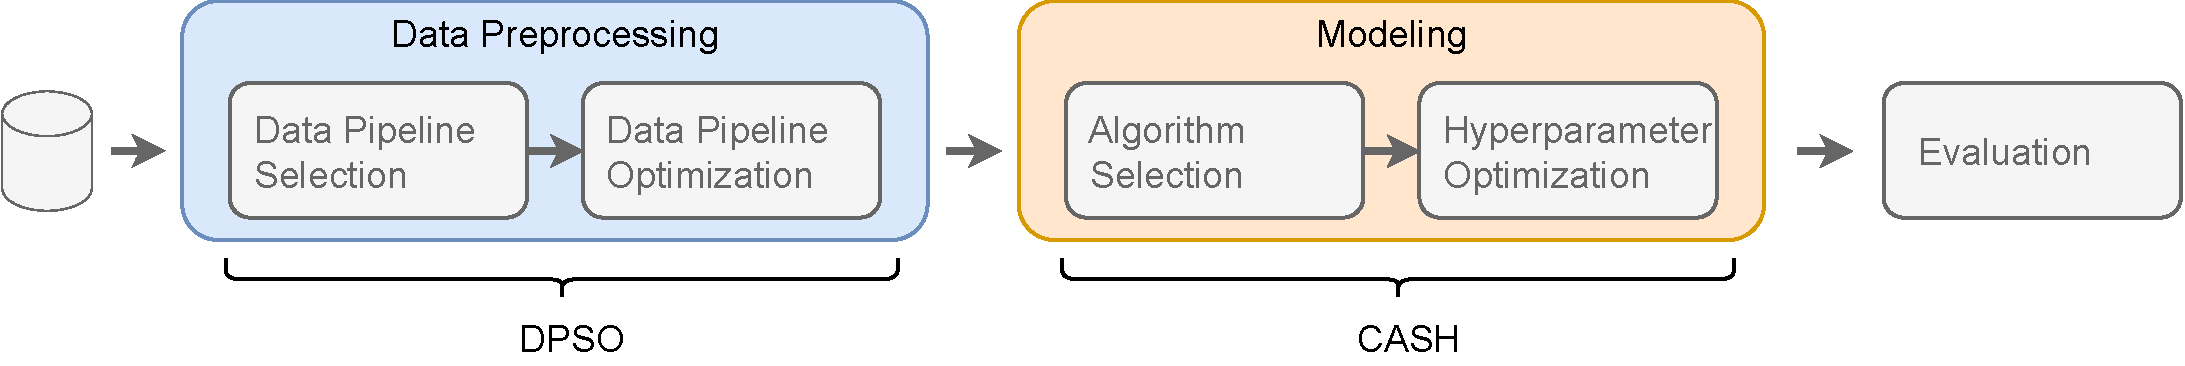
\includegraphics[width=1.0\textwidth]{chapters/data-centric/supervised/img/data-analytics-pipeline.pdf}
    \caption{Data analytics pipeline generation in a knowledge discovery process.}
    \label{effective-fig:data-analytics-pipeline}
\end{figure*}

To unleash the full potential of ML, data-centric AI focuses on shaping data according to the task and algorithm at hand.
With reference to the CRISP-DM process model,  \Cref{effective-fig:data-analytics-pipeline} summarizes the stages involved and the corresponding problems in the literature.
Firstly, data are extracted in a raw format from different sources and sifted out so that only a relevant subset is selected.
Next, during the pre-processing stage, the data pipeline selection and optimization (DPSO) \cite{Quemy19DOLAP} problem is tackled.
Once the data is transformed into the proper form, the modelling stage focuses on the combined algorithm selection and hyperparameter (CASH) optimization problem.
Finally, pipelines and algorithms
are evaluated over the dataset until an acceptable result is obtained.

It is well-known that the whole process requires expertise and is particularly challenging.
Particularly, data scientists spend most of their time on the heavily laborious work of pre-processing (i.e., around 50-80\% of the total \cite{Munson09Pre}).
Some AutoML frameworks \cite{auto_sklearn, mohr2018ml}, mix-in pre-processing during modelling optimization, but typically include very few transformations or do not consider all the necessary steps (e.g., imputation, rebalancing), thus in a way overlooking it.
Inspired from \cite{Munoz09DOLAP}, we contend that there is need for more data-centric techniques, encompassing all the steps of data pre-processing \cite{Vaisman14Book}.
Assistance is required in every phase \cite{Bilalli16IOTBD}.
By considering pre-processing as an integral component of the learning process, and carefully selecting and optimizing data pipelines, it is easy to obtain results that go beyond the ones obtained by only optimizing ML algorithms.

To briefly illustrate this, we perform an experiment on the well known \texttt{bank-marketing}\footnote{\url{https://archive.ics.uci.edu/ml/datasets/Bank+Marketing}} dataset, using HyperOpt \cite{HyperOptICML13} as an AutoML approach to optimize the parameters of three different ML algorithms, namely Naive Bayes (NB), K-Nearest Neighbor (KNN), and Random Forest (RF).
We provide an initial budget of 50 iterations for optimizing the hyperparameters of the algorithms, and after the 50th iteration, we fix the algorithm configuration to the best one achieved so far and start optimizing the pre-processing pipeline\footnote{This order is used only for the sake of illustration.}.
In \Cref{effective-fig:pre-processing-impact}, the ratio of the change in terms of accuracy (i.e., obtained after the i-th iteration to the baseline/default accuracy) is plotted against the number of different configurations visited by HyperOpt (i.e., iterations).
Observe that after the 11th iteration for NB and KNN, and after the 26th iteration for RF, the lines remain flat.
That is, from there on, no improvement is achieved by optimizing the hyperparameters of the algorithms until the 50th iteration is reached. At this point, a sudden jump is observed and the results start to improve again, going clearly beyond the ones obtained before, thanks to the optimizations performed now over the pre-processing pipeline.

\begin{figure}[t]
    \centering
    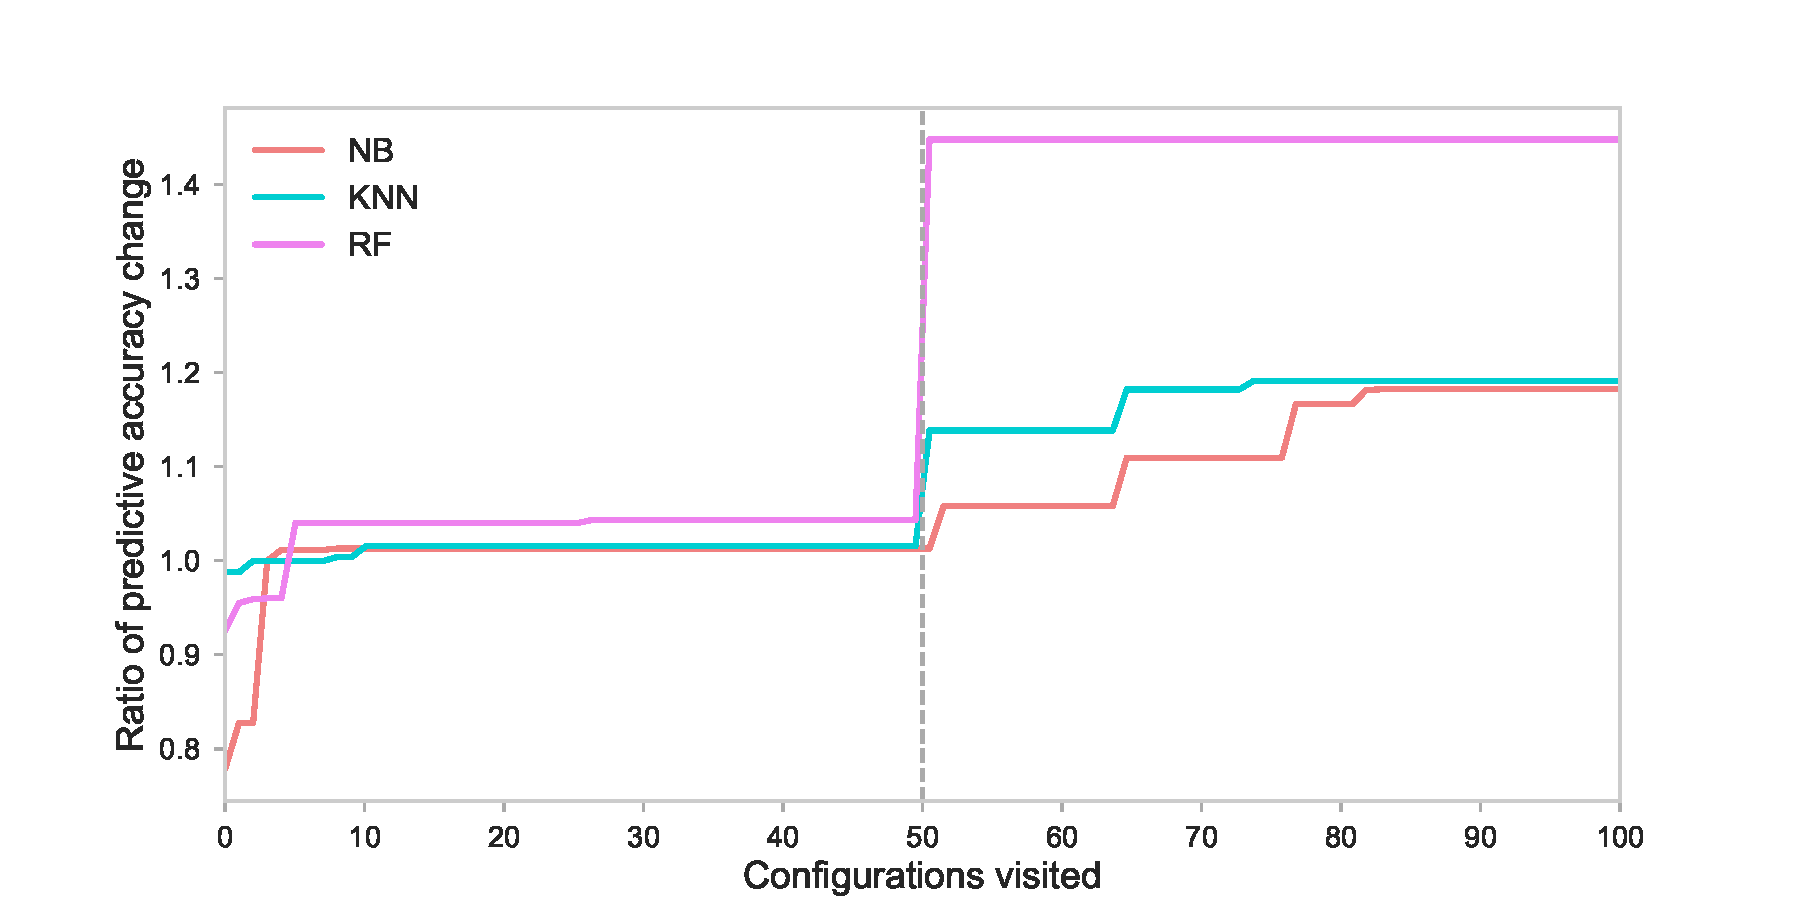
\includegraphics[width=0.7\textwidth]{chapters/data-centric/supervised/img/pre-processing-impact.pdf}
    \caption{Evolution of accuracy during the optimization process. The first 50 configurations optimize only the hyperparameters and after the 50th configuration, the pre-processing pipeline is optimized instead.}
    \label{effective-fig:pre-processing-impact}
\end{figure}

\paragraph{Challenges} Including pre-processing in the learning process heavily increases the search space, making the problem much harder.
DPSO entails two challenges that the data scientists have to undergo to find the most appropriate pipeline: (i) choose how to order the different pre-processing steps  (i.e., pipeline selection), and (ii) choose which transformations, with corresponding hyperparameters, should be adopted in the final implementation  (i.e., pipeline optimization).
To better distinguish between pipeline selection and its optimization, we follow the notation from \cite{Quemy20InfSystems}: a \textit{prototype} is the fixed and ordered sequence of pre-processing steps, its optimized instantiation of each transformation (with their hyperparameters) is known as \textit{executable pipeline}.

\paragraph{Contributions} The aim of this chapter is to study the two questions raised and propose a method for selecting effective pre-processing prototypes that, once optimized through some optimization technique (e.g., Bayesian optimization), improve the final result of the analysis.
To keep discussions and experiments simpler, we stick to supervised learning tasks.
The main contributions can be summarized as follows.
\begin{itemize}
    \item We empirically evaluate the impact of optimizing the exhaustive set of potential prototypes and find out that	there is no universal solution---i.e., prototype that works best for each dataset and algorithm considered.
    \item We define a method that given an ML algorithm and a set of pre-processing steps, is capable of generating the right order, obtaining effective pre-processing prototypes that are then instantiated via bayesian optimization.
    \item We suggest a meta-learning step (i.e., learning on top of learning) where the relationships between pre-processing transformations and dataset characteristics are learned in order to create rules that help with the initial instantiation of the prototypes.

	We exemplify our meta-learning study generating simple but not obvious and effective rules for two kinds of pre-processing steps, namely, Feature Engineering and Rebalancing.
    \item We perform a comprehensive evaluation by comparing the performance of optimizing prototypes generated following our method, and find out that:
    \begin{enumerate}
        \item with 24 times less time budget, our proposed pipelines obtain results whose median is above 90\% of the ones generated via exhaustive search.
        \item on average, in 73\% of the cases, splitting evenly the time budget between pre-processing and modelling outperforms the results of solely optimizing the latter.
    \end{enumerate}
	\item We deploy \textbf{AutoPrep}, a reproducibility framework for the automatic generation of effective pre-processing pipeline prototypes. Specifically, in \cite{}, we introduce: (i) a detailed reproducibility protocol, (ii) software, and (iii) datasets in a self-contained environment.
	The experiments were run on several machines and confirmed all the inishts in this chapter.
\end{itemize}

The remaining of this chapter is organized as follows:
\Cref{effective-sec:related-work} discusses the related work,
\Cref{effective-sec:methodology} presents our method of generating effective pipelines,
\Cref{effective-sec:evaluation} provides an extensive evaluation of the pipelines created using our proposed method and, finally, \Cref{effective-sec:conclusions} provides the conclusions and future work.


\section{Related Works}
\label{effective-sec:related-work}
At the beginning, the AutoML community followed the AI trend of contributing under a more algorithmic perspective, focusing on modelling---i.e., the resolution of the CASH problem.
Recently however, the direction has shifted towards designing systems that additionally or specifically provide user assistance in the data pre-processing step---i.e., solving the DPSO problem.
We can categorize works according to the optimization policy \cite{quemy2019data} they adopt.
On the one hand, some automate data pre-processing via split-like policies---i.e., addressing DPSO in isolation from CASH (\Cref{effective-ssec:dpso}).
On the other hand, some consider optimizing DPSO along with CASH, adopting a joint policy---data pre-processing in synergy with modelling (\Cref{effective-ssec:dpso-cash}).

\subsection{Optimization with Split-like Policies}
\label{effective-ssec:dpso}

In \cite{Quemy20InfSystems}, authors demonstrate the impact of optimizing the pre-processing pipelines, but considering only a single fixed prototype and only a few datasets.
However, as we have already seen (\Cref{effective-sec:eval-universal-pipeline}), a single fixed prototype cannot perform best for every dataset.

In PRESISTANT~\cite{presistant18CSI,presistant18CAISE,presistant19DKE}, authors tackled the problem of recommending pre-processing transformations to non-expert users.
They identify the pre-processing transformations and rank them in advance, based on their potential impact to the final analysis.
However, they do not consider pre-processing pipelines, but only single transformations, expecting that the analyst applies the process iteratively.

In ActiveClean \cite{ActiveClean16PVLDB}, authors define a method that aims at prioritizing the cleaning of records that are more likely to affect the results of the analysis, assuming that the latter belongs to the class of convex loss models (i.e., linear regression and SVMs).
Hence, instead of recommending the transformations to be applied, the system recommends the subset of data that needs to be cleaned at a given point.
The type of pre-processing to be applied is left to the user, assuming that the user is an expert.

In Learn2Clean~\cite{Berti19WWW}, based on a reinforcement learning technique, for a given dataset and an ML model, an optimal sequence of pre-processing transformations is generated so that the quality of the ML model is maximized.
Yet, similarly to~\cite{Quemy20InfSystems}, the pipeline prototype is fixed in advance.

In Alpine Meadow~\cite{Shang19SIGMOD}, authors follow a similar approach to ours in that they define two steps for the pre-processing phase. One, the so-called \textit{logical pipeline plan}, which is roughly equivalent to the \textit{prototype} defined in this work, and the second the \textit{physical pipeline plan} which translates to \textit{executable pipelines} used in this work.
The physical plan is generated through a combination of Bayesian optimization, meta-learning, and multi-armed bandits.
For the logical plans, they rely on rules but without clear evidence on how they are generated.
Moreover, it is not clear whether the logical plan is fixed as in \cite{Quemy20InfSystems} and if some further adjustment from the user is required.

\subsection{Optimization with a Joint Policy}
\label{effective-ssec:dpso-cash}
Auto-sklearn \cite{Feurer15AutoSklearn} is based on the popular Python library scikit-learn.
The authors, inspired by Auto-Weka, address the problem with the Sequential Model-based Algorithm Configuration (SMAC).
Furthermore, they improve the approach by adding a meta-learning phase (i.e., learning on top of learning) at the beginning and an ensemble technique at the end.
Meta-learning leverages previous ML experiments and learns promising configurations to warm-start (i.e., boost the convergence) the Bayesian Optimization.
Ensemble techniques merge predictions from multiple ML models to statistically outperform the base models.
Yet, they consider a small set of transformations and also consider a single fixed prototype.

TPOT \cite{Olson16Tpot} is a tree-based pipeline optimization tool using genetic programming while requiring little to no expertise from the user.
In TPOT however, they only consider one transformation inside the optimization process (i.e., Feature Engineering).

ML-Plan \cite{mohr2018ml} uses hierarchical planning, a particular form of AI planning, to propose a solution to both the pre-processing and the modeling phases.
As in context-free grammars, there are complex tasks (non-terminal symbols) that are derived as long as primitive tasks (terminal symbols) are not obtained.
Typically, standard graph search algorithms (e.g., depth-first search, best-first search, etc.) are employed to solve such problems.
ML-Plan successively creates solutions in a global search instead of changing given solutions in a local search. However, due to the problem constraints, they adopt a randomized best-first search, randomly choosing the solution path.

AutoBazaar \cite{AutoBazaar} is a Python open-source tool.
Like in ML-Plan \cite{mohr2018ml}, both pre-processing and modeling phases are covered.
Here the last step of a prototype is the machine learning algorithm.
The approach involves two different steps.
Firstly, a \textit{catalog} proposes a collection of prototypes (with an ML algorithm as last step) based on the task and the dataset itself.
Secondly, the optimization process starts tuning the prototypes until either the time budget is expired or the prototypes are all optimized.
In particular, a \textit{selector} and a \textit{tuner} work in synergy.
The former decides which prototype should be optimized next.
Such a task is treated as a multi-armed bandit problem.
As to the tuner, bayesian optimization is chosen.
At the end, the prototype that achieved the higher accuracy is elected.
However, AutoBazaar strictly depends on the catalog.
Such a component memorizes all the possible primitives and supported tasks.
The prototypes are hard-coded for each task.
Thus, it is neither flexible nor maintainable.
If a task is not implemented, the approach cannot suggest a solution.

To summarize, full automation of data analytics has been the ultimate goal of many research works.
Yet, such automation has shown to be computationally expensive, mainly due to the search space involved (i.e., pre-processing and mining operators).
Therefore, the usability of these approaches in realistic scenarios is sometimes limited.
Our approach of finding a set of effective prototypes can be seen as complementary to these solutions, since it helps in pruning the large space and guiding the search, hence reducing their cost.

\section{Effective Data Pre-processing Pipeline Generation}
\label{effective-sec:methodology}

We aim to find the best data pipeline (i.e., with higher performance) for the dataset $\altmathcal{D}$ and the ML algorithm $A$ considered, hence solving DPSO.
Let us refresh the formalization of interest.

Each transformation $T$ exposes a set of $K$ hyperparameters, producing the Cartesian product $\Lambda_T = \Lambda_1 \times \dots \times \Lambda_K$.
A pre-processing \textit{step} $S$ can be instantiated from several alternative transformations, hence $\Lambda_S = \Lambda_{T_1} \cup \ldots \cup \Lambda_{T_{|S|}} \cup \lambda_s$, with $\lambda_s$ a new root-hyperparameter that selects the transformation.
The problem exacerbates when steps are combined together into data pipelines.
Indeed, the complete search space for our optimization problem is defined as $\Lambda_P = \Lambda_{S_1} \times \ldots \times \Lambda_{S_{|P|}} \times \lambda_p$, with $\lambda_p$ as yet another root-hyperparameter to select -- this time -- the order between the transformations (translating into the disjoint union of all partial permutations).

To mitigate the problem's complexity, we distinguish between pipeline selection and its optimization.
Specifically, following the notation from \cite{quemy2019data}:
pipeline selection aims at finding promising \textit{prototypes}, i.e. fixed and ordered sequence of pre-processing steps, pipeline optimization instantiates the best \textit{executable pipeline}, i.e. assigning a transformation (along with the hyperparameters) to each pre-processing step.

\begin{figure*}[t]
    \centering
    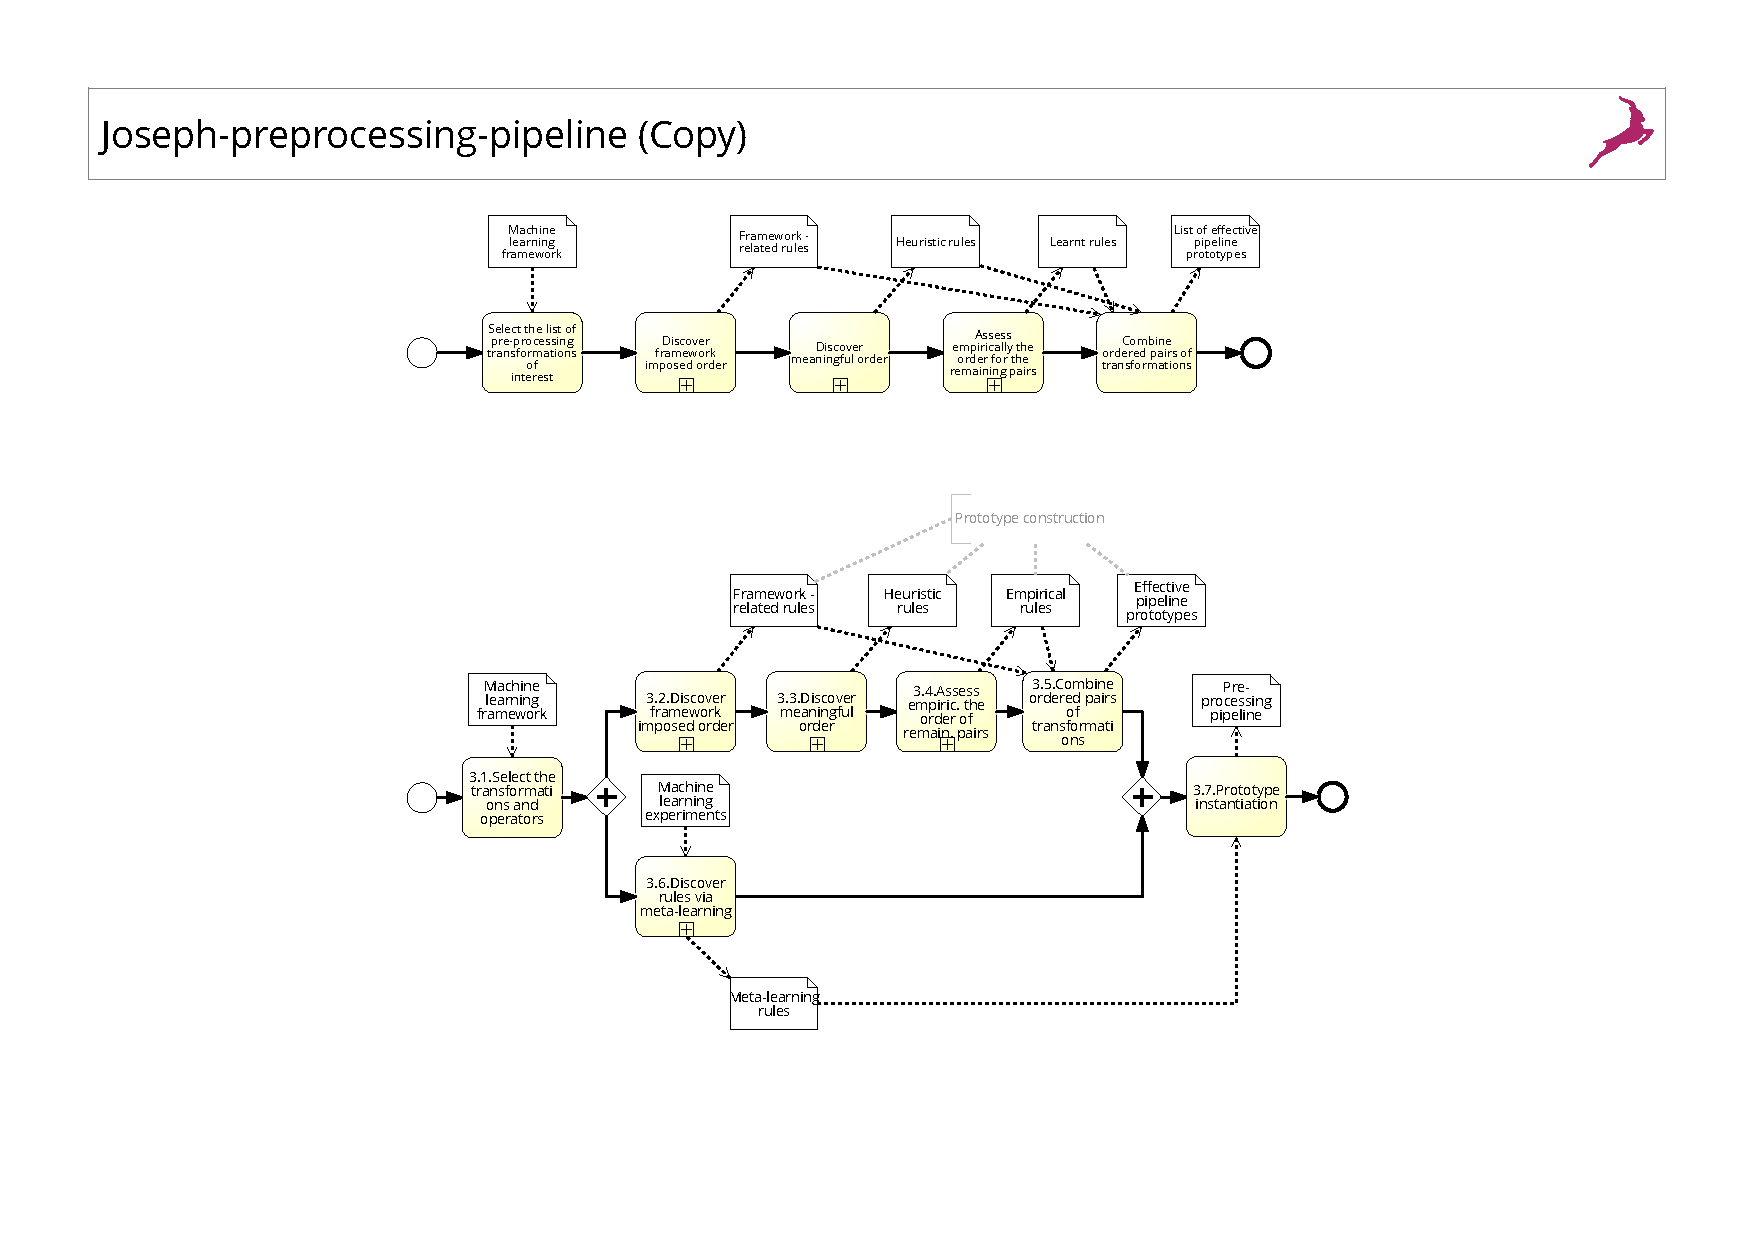
\includegraphics[width=1.0\textwidth]{chapters/data-centric/supervised/img/bpmn.pdf}
    \caption{A method for generating effective pre-processing pipelines}
    \label{effective-fig:methodology}
\end{figure*}

\Cref{effective-fig:methodology} sketches the proposed methodology, some of the phases are generic and thus can be applied regardless of the context, and yet others are specific (i.e., ML framework or dataset characteristics).
According to \cite{Quemy20InfSystems}, we break the combinatorial problem into two workflows: (i) studying pre-processing steps in pairs for generating effective prototypes and then (ii) feeding them to an optimizer (e.g., we use the SMBO \cite{HyperOptICML13} variant) for their actual instantiation.

\paragraph{Effective Prototypes Generation} The proposed method starts with the selection of the ML library (\Cref{effective-ssec:select-framework}).
This allows to consider solely the steps for which their implementation is available.
Besides, with such a choice, we are also provided with a set of \textit{framework-related rules} (\Cref{effective-ssec:rules-framework}), constraining the possible orderings of the steps (e.g., in scikit-learn, Imputation has to be the first step in the prototype).
These rules are in the form of precedences of pre-processing steps (i.e. orderings that involve two steps at a time;  e.g., Imputation before Normalization).
Next, the flow on top continues with a study
aiming to find the correct/meaningful orderings according to
the behavior of the transformations in each step.
As a result, this generates a set of \textit{heuristic rules} (\Cref{effective-ssec:rules-heuristics}) that restrict the space of possible precedences.
Afterward, for the pairs for which an order cannot be clearly devised, an additional empirical study is proposed.
This study relies on a test bed of representative datasets.
The output is a set of \textit{empirically-learned rules} (\Cref{effective-ssec:rules-learned}) that determines yet other precedences, namely promising orderings that would potentially positively impact the final result of the analysis.
However, even after this phase, for some pairs of pre-processing steps, a precedence order may not be found.
These are pairs for whom the order is relevant but cannot be decided in advance, thus all their permutations need to be present.
Finally, a step of composition follows  (\Cref{effective-ssec:composition}), where given the overall set of devised rules (i.e., \textit{framework-related}, \textit{heuristic} and \textit{empirically-learned}), the pre-processing steps are composed into a set of valid and potentially effective prototypes.

More formally, when combining two different pre-processing steps, it is important to check if, (i) the input and output types of the steps are compatible, (ii) the combination makes sense, and (iii) the combination provides good results for the analysis.
As a result, when chaining a pair of steps, the following precedence relationships arise:
\begin{enumerate}
    \item Compatible/Incompatible. Depending on whether the representation output of the first step is accepted as the representation input of the second one (compatible), or not (incompatible).
    \item Meaningful/Meaningless. Depending on whether the precedence between them makes sense based on generic knowledge (i.e., based on the literature) over the behaviour of transformations (meaningful), or not (meaningless).
    \item Promising/Unpromising. Depending on whether the precedence between them is expected to provide a positive impact on the final result of the analysis (promising), or not (unpromising).
\end{enumerate}

Attending to the relationships between its steps, a prototype can be described as either \textit{compatible}, \textit{well-formed}, or \textit{effective}.
A prototype is defined to be \textit{compatible} if all its precedence relationships are available in the ML framework at hand.
It is defined as \textit{well-formed} if all its precedence relationships are both compatible and meaningful.
Finally, it is defined as \textit{effective} if all its precedence relationships are compatible, meaningful, and promising at the same time.
In fact, the goal of this flow is to find \textit{effective prototypes}.

\paragraph{Warm-starting via Meta-learning} Once the prototype is constructed, the flow running in parallel is proposed to help with its instantiation.
It consists of a meta-learning step  (\Cref{effective-ssec:meta-learning}), where a set of ML experiments (e.g., pre-processing and classification algorithm runs) are used as training data to predict promising transformations for a pre-processing step.
These rules extract knowledge from past experiments and are complementary to the rules obtained in the first flow.
This practice is called warm-starting,
They would be used, for example, to ease the cold start problem in the prototype instantiation phase  (\Cref{effective-ssec:prototype-insta}).

We propose a generic methodology.
However, to keep the reader from losing, we will illustrate our use case and corresponding findings along with the explanation of the methodology.

\subsection{Selection of Data Pre-Processing Steps and Transformations}
\label{effective-ssec:select-framework}

The first task in the process consists of selecting the data pre-processing steps and their available transformations according to the selected ML library.

\paragraph{Use case}
For our experiments, we selected the pre-processing steps, transformations and hyperparameters from those available in the scikit-learn library\footnote{\url{https://scikit-learn.org}} (\Cref{effective-tbl:transformations}).
\textit{Input} denotes the compatible feature type for a given pre-processing step and can be continuous (CO) -- when it represents measurements on some continuous scale -- or categorical (CA)---when it represents information about some categorical or discrete characteristics.
Similarly, \textit{Output} denotes the type of the features after a pre-processing step is applied.

\begin{itemize}[noitemsep,topsep=0pt]
\item{Encoding ($E$).} The process of transforming categorical features into continuous ones (here, we refer solely to the encoded representation, not the semantic).
\item{Normalization ($N$).} The process of normalizing continuous features such that their values fall in the same range.
\item{Discretization ($D$).} The process of transforming continuous features into categorical ones.
\item{Imputation ($I$).} The process of imputing missing values.
\item{Rebalancing ($R$).} The process of adjusting the class distribution of a dataset (i.e. the ratio between the different classes/categories represented).
\item{Feature Engineering ($F$).} The process of defining the set of relevant features to be used in model training.
\end{itemize}

Finally, \textit{transformations} denotes the actual instantiation for the step, and it can be tuned using its \textit{hyperparameters}.


\begin{table}[!t]
\renewcommand{\arraystretch}{0.3}
\footnotesize
\caption{List of transformations applicable to categorical or continuous data types.}
\centering
\begin{threeparttable}

\begin{tabular}{@{}p{30mm}lll>{\ttfamily}l@{}}
\toprule
Pre-processing Step& Input & Output & Transformation & \textnormal{Hyperparameters}
\\	\cmidrule[.1em]{1-5}

Encoding ($E$)  & CA & CO & Ordinal & -  \\ \cmidrule[.05em]{4-5} & & & One Hot & - \\
\cmidrule[.1em]{1-5}

Normalization ($N$) & CO & CO & Standard Scaler & with\_mean:[True,False]\\ \cmidrule[.05em]{4-5} & & & & with\_std:[True,False] \\ \cmidrule[.05em]{4-5}
&  &  & Power Transform & -\\ \cmidrule[.05em]{4-5}
&  &  & MinMax Scaler & -\\ \cmidrule[.05em]{4-5}
&  &  & Robust Scaler & quantile\_range:[(25,75),(10,90),(5,95)]\\ \cmidrule[.05em]{4-5} & & & & with\_centering:[True,False]\\ \cmidrule[.05em]{4-5} & & & & with\_scaling:[True,False] \\
\cmidrule[.1em]{1-5}

Discretization ($D$) & CO & CA & KBins & n\_bins:[3,5,7]\\ \cmidrule[.05em]{4-5} & & & & encode:[`onehot',`onehot-dense',`ord.']\\ \cmidrule[.05em]{4-5} & & & & strategy:[`uniform',`quant.',`kmeans']\\	\cmidrule[.05em]{4-5}
&  &  & Binarization  & threshold: [0, 0.5, 2, 5]\\	\cmidrule[.1em]{1-5}

Imputation ($I$) & CA/CO & CA/CO  & Univariate & strategy:[`most\_freq.','constant'] \\	\cmidrule[.05em]{4-5}
 & &  & Multivariate & initial\_strategy:[`most\_freq',`const.']\\ \cmidrule[.05em]{4-5} & & & & order:[`asc',`dsc',`rom',`arab',`rand'] \\	\cmidrule[.1em]{1-5}

Rebalancing ($R$)* &CA/CO  & CA/CO & Near Miss & n\_neighbors:[1,2,3]\\ \cmidrule[.05em]{4-5}
%&  &  & \textcolor{red}{Condensed KNN} & \textcolor{red}{n\_neighbors:[1,2,3]} \\ \cmidrule[.05em]{4-5}
&  &  & SMOTE & k\_neighbors:[5,6,7]\\	\cmidrule[.1em]{1-5}

Feat. Eng. ($F$) & CA/CO & CA/CO & PCA & n\_components:[1,2,3,4]\\ \cmidrule[.05em]{4-5}
&  &  & Select K Best & k:[1,2,3,4]\\ \cmidrule[.05em]{4-5}
&  &  & PCA + Select K Best  & n\_components:[1,2,3,4]
\\ \cmidrule[.05em]{4-5} & & & & k:[1,2,3,4]\\	\bottomrule%\cmidrule[.1em]{1-5}
\end{tabular}
\begin{tablenotes}
\footnotesize
\item CA - categorical, CO - continuous.
\item *All transformations except Rebalancing are taken from scikit-learn.
\end{tablenotes}
\end{threeparttable}
\label{effective-tbl:transformations}
\end{table}

\begin{table*}[!t]
    \caption{
        Precedence order between pairs of pre-processing steps, represented independently for each phase.
        }
    \renewcommand{\arraystretch}{0.3}
    \footnotesize
    \begin{center}
    \subfloat[Compatible precedence.]{
    \begin{tabular}{@{}lcccccc}
    \toprule
     & $\boldsymbol{E}$ & $\boldsymbol{N}$ & $\boldsymbol{D}$ & $\boldsymbol{I}$ & $\boldsymbol{R}$ & $\boldsymbol{F}$
    \\	\cmidrule[.1em]{1-7}
    $\boldsymbol{E}$ & \cellcolor{gray!25} & \texttt{1} & \texttt{1} & \texttt{\texttt{0}} & \texttt{1} & \texttt{1} \\	\cmidrule[.1em]{1-7}
    $\boldsymbol{N}$ & \texttt{0} & \cellcolor{gray!25}  & \texttt{0} & \texttt{0} & \texttt{0} & \texttt{0} \\	\cmidrule[.1em]{1-7}
    $\boldsymbol{D}$ & \texttt{0} & \texttt{0} & \cellcolor{gray!25}  & \texttt{0} & \texttt{0} & \texttt{0} \\	\cmidrule[.1em]{1-7}
    $\boldsymbol{I}$ & \texttt{1} & \texttt{0} & \texttt{1} & \cellcolor{gray!25}  & \texttt{1} & \texttt{1} \\	\cmidrule[.1em]{1-7}
    $\boldsymbol{R}$ & \texttt{0} & \texttt{0} & \texttt{0} & \texttt{0} & \cellcolor{gray!25}  & \texttt{0} \\	\cmidrule[.1em]{1-7}
    $\boldsymbol{F}$ & \texttt{0} & \texttt{0} & \texttt{0} & \texttt{0} & \texttt{0} & \cellcolor{gray!25}
    \\	\bottomrule
    \end{tabular}}
    \qquad% --- set horizontal distance between tables here
    \subfloat[Meaningful precedence.]{%
    \begin{tabular}{@{}lcccccc}
    \toprule
    & $\boldsymbol{E}$ & $\boldsymbol{N}$ & $\boldsymbol{D}$ & $\boldsymbol{I}$ & $\boldsymbol{R}$ & $\boldsymbol{F}$
    \\	\cmidrule[.1em]{1-7}
    $\boldsymbol{E}$ & \cellcolor{gray!25} & \texttt{0} & \texttt{0} & \texttt{0} & \texttt{0} & \texttt{0} \\	\cmidrule[.1em]{1-7}
    $\boldsymbol{N}$ & \texttt{0} & \cellcolor{gray!25}  & \texttt{X} & \texttt{0} & \texttt{1} & \texttt{0} \\	\cmidrule[.1em]{1-7}
    $\boldsymbol{D}$ & \texttt{0} & \texttt{X} & \cellcolor{gray!25}  & \texttt{0} & \texttt{0} & \texttt{0} \\	\cmidrule[.1em]{1-7}
    $\boldsymbol{I}$ & \texttt{1} & \texttt{1} & \texttt{1} & \cellcolor{gray!25}  & \texttt{1} & \texttt{1} \\	\cmidrule[.1em]{1-7}
    $\boldsymbol{R}$ & \texttt{0} & \texttt{0} & \texttt{0} & \texttt{0} & \cellcolor{gray!25}  & \texttt{0} \\	\cmidrule[.1em]{1-7}
    $\boldsymbol{F}$ & \texttt{0} & \texttt{0} & \texttt{0} & \texttt{0} & \texttt{0} & \cellcolor{gray!25}
    \\	\bottomrule
    \end{tabular}}
    \qquad% --- set horizontal distance between tables here
    \subfloat[Promising precedence.]{%
    \begin{tabular}{@{}lcccccc}
    \toprule
    & $\boldsymbol{E}$ & $\boldsymbol{N}$ & $\boldsymbol{D}$ & $\boldsymbol{I}$ & $\boldsymbol{R}$ & $\boldsymbol{F}$
    \\	\cmidrule[.1em]{1-7}
    $\boldsymbol{E}$ & \cellcolor{gray!25} & \texttt{0} & \texttt{0} & \texttt{0} & \texttt{0} & \texttt{0} \\	\cmidrule[.1em]{1-7}
    $\boldsymbol{N}$ & \texttt{0} & \cellcolor{gray!25} & \texttt{0} & \texttt{0} & \texttt{0} & \texttt{1} \\	\cmidrule[.1em]{1-7}
    $\boldsymbol{D}$ & \texttt{0} & \texttt{0} & \cellcolor{gray!25} & \texttt{0} & \texttt{0} & \texttt{1} \\	\cmidrule[.1em]{1-7}
    $\boldsymbol{I}$ & \texttt{0} & \texttt{0} & \texttt{0} & \cellcolor{gray!25} & \texttt{0} & \texttt{0} \\	\cmidrule[.1em]{1-7}
    $\boldsymbol{R}$ & \texttt{0} & \texttt{0} & \texttt{0} & \texttt{0} & \cellcolor{gray!25} & \texttt{0} \\	\cmidrule[.1em]{1-7}
    $\boldsymbol{F}$ & \texttt{0} & \texttt{0} & \texttt{0} & \texttt{0} & \texttt{0} & \cellcolor{gray!25}
    \\	\bottomrule
    \end{tabular}}
    \end{center}
    \begin{tablenotes}
    \centering
    \scriptsize
    \item$\boldsymbol{E}$ - Encoding; $\boldsymbol{N}$ - Normalization; $\boldsymbol{D}$ - Discretization; $\boldsymbol{I}$ - Imputation; $\boldsymbol{R}$ - Rebalancing; $\boldsymbol{F}$ - Feature Engineering. \item \texttt{1} - a precedence edge exists between the row and the column, \texttt{0} - a precedence edge does not exist between the row
    \item and the column, \texttt{X} - the combination is meaningless.
    \end{tablenotes}
    \label{effective-tbl:rules}
    \end{table*}

\subsection{Extraction of Compatible Precedences}
\label{effective-ssec:rules-framework}

Once the implementation framework is selected, one needs to study it and see if there exist constraints that limit the interaction between the pre-processing steps.
For instance, applying a step may actually invalidate the application of another one, because the compatibility of them is dependent on the selected ML framework.
We aim at detecting a set of implicit rules that are shown through an adjacency matrix, corresponding to a precedence graph as those in \Cref{effective-tbl:rules}.
Each cell $a_{ij}$ denotes a precedence relationship between the row $i$ and column $j$.
Hence, \texttt{1} means that an edge exists between the transformation in the row and the transformation in the column, whereas \texttt{0} means that such an edge does not exist, hence a precedence order is not established for that pair.

\paragraph{Use case}
We studied the pre-processing steps implemented in Scikit-learn, the discovered rules are shown through the adjacency matrix in \Cref{effective-tbl:rules}a.
For example, most Scikit-learn steps cannot be applied in the presence of missing values.
This is why in every pair of them where Imputation is involved, except the one with Normalization\footnote{Normalization transformations are the only ones that Scikit-learn can apply on datasets with missing values.}, Imputation goes first.
Furthermore, Scikit-learn steos are applied only to all compatible features of a given dataset.
Generally, categorical features are physically represented as strings and continuous features as numbers.
However, a transformation that is meant to be applied, say to continuous features, cannot be applied over a dataset that contains both continuous and categorical features (i.e., a dataset containing both numbers and strings); Scikit-learn cannot deal with arrays of mixed types.
In that case, all the categorical features need to be encoded into numeric representations, even if they represent a categorical value.
That is, a value can be a number but represent a category.
This is what happens when Normalization and Discretization are meant to be applied to a dataset containing mixed types of features.
In order for them to be applied to datasets of mixed types, an Encoding transformation needs to be applied first.
A similar constraint is imposed when considering Rebalancing and Feature Engineering, since these steps do not accept inputs containing strings (i.e., representing a categorical type).
For the rest of the pairs, there are no constraints imposed by the framework, thus any ordering is permitted, reflected by a \texttt{0} in \Cref{effective-tbl:rules}a.
The graph obtained in this case exclusively corresponds to the limitations of Scikit-learn (as a matter of fact, if another framework were to be chosen, it may have looked differently).

\subsection{Discovery of Well-formed Precedences}
\label{effective-ssec:rules-heuristics}
Once we have derived precedences based on the constraints of the framework, we can study the precedence independently and find \textit{meaningful pairs}.
That is, for every given pair, we want to find the relative order based on generic domain-independent knowledge (i.e., literature) about pre-processing steps and their applicability.
To this end, some of the constraints imposed by the framework may be contradicted here, but this is resolved in the last step of the proposed method (\Cref{effective-ssec:composition}).
Briefly, in a combination where Imputation is involved, it is advised to apply Imputation first.
Next, Encoding makes sense to be combined in any order with the rest of the transformations, except Imputation.
Combining Discretization with Normalization does not make sense, due to the fact that after the Discretization step, continuous features are transformed into categorical ones, and hence Normalization cannot be applied.
Similarly, applying Normalization first, changes the scale of the values and hence impacts the Discretization step.
Finally, a meaningful precedence can be derived when combining Normalization with Rebalancing.
In this case, Normalization should be applied first, since otherwise Rebalancing would impact the scale of the values to be normalized.

\paragraph{Use case}
\Cref{effective-tbl:rules}b shows the heuristic rules obtained considering domain-independent knowledge about the steps \cite{BookExploratoryDM03Dasu}.
In comparison with the results from \Cref{effective-tbl:rules}a, observe that the constraints on the Imputation still hold: when combining it ith another step, Imputation should go first.
This time even when combining it with Normalization---note the difference with \Cref{effective-tbl:rules}a.
The constraints of Encoding are however not present in \Cref{effective-tbl:rules}a, hence not considering the framework, Discretization combined with Encoding is a meaningful combination---when a mixed type dataset is considered, but incompatible from the point of view of Scikit-learn.

\subsection{Empirical-learning of Promising Precedences}
\label{effective-ssec:rules-learned}

The two previously proposed phases (i.e., \textit{framework-related} and \textit{heuristic rules}), do not guarantee that each pair of steps will obtain a precedence order.
Therefore, for those cases left out, a third viewpoint should be considered.
That of learning a promising order by empirically studying the impact of the combinations on the final result of the analysis, using different supervised problems in the training.
For every selected pair of pre-processing steps, for a given ML algorithm, we propose to check which order of the pair improves most the performance (e.g., accuracy) of the algorithm over a set of datasets (preferably from different domains).
Like this, for each dataset, we can get a precedence order that gives better results (i.e., promising precedence) in terms of the loss.


\begin{algorithm*}[!h]
	\caption{Find a promising prototype for steps $S_1$ and $S_2$}
	\label{effective-alg:learned-rules}
	\begin{algorithmic}[1]
		\Require $\altmathcal{D}_{train}$, $\altmathcal{D}_{valid}$, $A$, $\altmathcal{L}$ $S_1$, $S_2$ \Comment{dataset split for train and validation, classification algorithm, loss function, two different pre-processing steps}
		% \Require \indent$S_1\rightarrow S_2$, $S_2 \rightarrow S_1$ \Comment{precedence orders of a pair of transformations}
		\State $\altmathcal{L}_{\varnothing} = \altmathcal{L}(A(\altmathcal{D}_{train}), \altmathcal{D}_{valid})$ \Comment{get baseline performance of algorithm $A$ on $\altmathcal{D}$}
		\State $P_1 = \langle S_1, S_2 \rangle, P_2 = \langle S_2, S_1 \rangle$ \Comment{define two prototypes}
		\State $P_{1_{\lambda}} = SMBO(\langle P_1, A \rangle(\altmathcal{D}_{train}), \altmathcal{D}_{valid})$ \Comment{optimize the 1st prototype and get the best pipe}
		\State $\altmathcal{L}_{P_1} = \altmathcal{L}(\langle P_{1_{\lambda}}, A \rangle(\altmathcal{D}_{train}), \altmathcal{D}_{valid})$ \Comment{get the corresponding loss}
		\State $P_{2_{\lambda}} = SMBO(\langle P_2, A \rangle(\altmathcal{D}_{train}), \altmathcal{D}_{valid})$
		\Comment{optimize the 2nd prototype and get the best pipe}
		\State $\altmathcal{L}_{P_2} = \altmathcal{L}(\langle P_{2_{\lambda}}, A \rangle(\altmathcal{D}_{train}), \altmathcal{D}_{valid})$ \Comment{get the corresponding loss}
		% \State $[pipeline_{S_2\rightarrow S_1},acc_{S_2\rightarrow S_1}] = SMBO(S_2\rightarrow S_1,d, a)$
		% \Comment{get pipeline and accuracy for $S_2\rightarrow S_1$}
		% \If{\textit{IsValid}($acc_{S_1\rightarrow S_2},acc_{S_2\rightarrow S_1},acc_{baseline}$)}
		\If{$P_{1_{\lambda}}, P_{2_{\lambda}}$ are valid w.r.t. $\altmathcal{L}_{\varnothing}, \altmathcal{L}_{P_1}, \altmathcal{L}_{P_2}$}
        \Comment{see \Cref{effective-tbl:validation-rules} for the rules applied}
        \State \Return Best of $P_1$ and $P_2$
        \Comment{see column \textit{Winner prototype} in \Cref{effective-tbl:validation-rules}}
		\Else
		\State \Return $\varnothing$
		\EndIf
	\end{algorithmic}
\end{algorithm*}

\subsubsection{Experimental Learning Design}
To find a promising precedence order between a given pair of pre-processing steps $S_1$ and $S_2$, we propose \Cref{effective-alg:learned-rules}.
Let us consider a dataset split into $\altmathcal{D}_{train}$ and $\altmathcal{D}_{valid}$, a ML algorithm $A$, and a loss function $\altmathcal{L}$.
We first calculate $\altmathcal{L}_{\varnothing}$ as the loss of the ML algorithm $A$ over the original non-transformed dataset (line 1).
Afterward, to compute the impact of each possible prototype $P_1$ and $P_2$ (line 2), we leverage SMBO to find their optimized executable pipelines (line 3 and 5), and the losses of the ML algorithm (with default configuration) over the datasets transformed using the respective pipelines (line 4 and 6).
Based on the comparison between the respective optimized pipelines, we get the winner (line 7).
However, beforehand (line 6), we perform a validity check.
This is because when optimizing a pre-processing pipeline, SMBO may not instantiate a step with no transformation at all (i.e., represented with a $\varnothing$ symbol).
Hence, given a pair of pre-processing steps, where one or both of them may not be instantiated, SMBO may generate 16 possible scenarios.
They are listed in \Cref{effective-tbl:validation-rules}, and make up the validation rules for \Cref{effective-alg:learned-rules}.

\begin{table*}[t]
	\footnotesize
	\centering
	\begin{threeparttable}
	\caption{
		Validation rules.
		}
	\begin{tabular}{lp{2.3cm}p{2.3cm}p{2cm}p{2cm}p{2.5cm}}
	\toprule
	Nr. & Ex. Pipeline $P_{1_{\lambda}}$ & Ex. Pipeline $P_{2_{\lambda}}$ & Valid result & Valid score & Winner prototype\\\toprule
			1. &$\langle \varnothing, \varnothing \rangle$ & $\langle \varnothing, \varnothing \rangle$ & Draw          & $\altmathcal{L}_{\varnothing}$ &  Baseline \\ \hline
			2. &$\langle \varnothing, \varnothing \rangle$ & $\langle S_{2_{\lambda}}, \varnothing \rangle$ & Draw          & $\altmathcal{L}_{\varnothing}$ & Baseline \\ \hline
			3. &$\langle \varnothing, \varnothing \rangle$ & $\langle \varnothing, S_{1_{\lambda}} \rangle$ & Draw          & $\altmathcal{L}_{\varnothing}$ & Baseline \\ \hline
			\multirow{2}{*}{4.} &\multirow{2}{*}{$\langle \varnothing, \varnothing \rangle$} & \multirow{2}{*}{$\langle S_{2_{\lambda}}, S_{1_{\lambda}} \rangle$} & Draw & $\altmathcal{L}_{\varnothing}$ & Baseline \\
			& & & $P_{2_{\lambda}}$ & $\altmathcal{L}_{P_2}$ & $P_2$\\ \hline
			5. & $\langle \varnothing, S_{2_{\lambda}} \rangle$ & $\langle \varnothing, \varnothing \rangle$ & Draw          & $\altmathcal{L}_{\varnothing}$ & Baseline \\ \hline
			\multirow{3}{*}{6.} & \multirow{3}{*}{$\langle \varnothing, S_{2_{\lambda}} \rangle$} & \multirow{3}{*}{$\langle S_{2_{\lambda}}, \varnothing \rangle$} & Draw &  \multirow{3}{*}{$\altmathcal{L}_{S_2}$}  & $S_2$ \\
			& & & $P_{1_{\lambda}}$ & & $S_2$ \\
			& & & $P_{2_{\lambda}}$ & & $S_2$ \\ \hline
			7. &$\langle \varnothing, S_{2_{\lambda}} \rangle$ & $\langle \varnothing, S_{1_{\lambda}} \rangle$ & Draw & $\altmathcal{L}_{S_2}$ or $\altmathcal{L}_{S_1}$ & $S_{1}\,or\, S_2$ \\ \hline
			\multirow{2}{*}{8.} & \multirow{2}{*}{$\langle \varnothing, S_{2_{\lambda}} \rangle$} & \multirow{2}{*}{$\langle S_{2_{\lambda}}, S_{1_{\lambda}} \rangle$} & Draw & $\altmathcal{L}_{S_2}$ & $S_2$\\
			& & & $P_{2_{\lambda}}$ & $\altmathcal{L}_{P_2}$ & $P_2$ \\ \hline
			9. & $\langle S_{1_{\lambda}}, \varnothing \rangle$ & $\langle \varnothing, \varnothing \rangle$ & Draw & $\altmathcal{L}_{\varnothing}$ & Baseline \\ \hline
			10. & $\langle S_{1_{\lambda}}, \varnothing \rangle$ & $\langle S_{2_{\lambda}}, \varnothing \rangle$ & Draw & $\altmathcal{L}_{S_1}$ or $\altmathcal{L}_{S_2}$ & $S_{1}\,or\, S_2$ \\ \hline
			\multirow{3}{*}{11.} & \multirow{3}{*}{$\langle S_{1_{\lambda}}, \varnothing \rangle$} & \multirow{3}{*}{$\langle \varnothing, S_{2_{\lambda}} \rangle$} & Draw & \multirow{3}{*}{$\altmathcal{L}_{S_1}$} & $S_1$\\
			& & & $P_{1_{\lambda}}$ & & $S_1$\\
			& & & $P_{2_{\lambda}}$ & & $S_1$\\ \hline
			\multirow{2}{*}{12.} & \multirow{2}{*}{$\langle S_{1_{\lambda}}, \varnothing \rangle$} & \multirow{2}{*}{$\langle S_{2_{\lambda}}, S_{1_{\lambda}} \rangle$} & Draw & $\altmathcal{L}_{S_1}$  & $S_1$\\
			& & & $P_{2_{\lambda}}$ & $\altmathcal{L}_{P_2}$ & $P_2$ \\ \hline
			\multirow{2}{*}{13.} & \multirow{2}{*}{$\langle S_{1_{\lambda}}, S_{2_{\lambda}} \rangle$} & \multirow{2}{*}{$\langle \varnothing, \varnothing \rangle$} & Draw & $\altmathcal{L}_{\varnothing}$  & Baseline\\
			& & & $P_{1_{\lambda}}$ & $\altmathcal{L}_{P_1}$ & $P_1$ \\ \hline
			\multirow{2}{*}{14.} & \multirow{2}{*}{$\langle S_{1_{\lambda}}, S_{2_{\lambda}} \rangle$} & \multirow{2}{*}{$\langle S_{2_{\lambda}}, \varnothing \rangle$} & Draw & $\altmathcal{L}_{S_2}$ & $S_2$\\
			& & & $P_{1_{\lambda}}$ & $\altmathcal{L}_{P_1}$  & $P_1$ \\ \hline
			\multirow{2}{*}{15.} & \multirow{2}{*}{$\langle S_{1_{\lambda}}, S_{2_{\lambda}} \rangle$} & \multirow{2}{*}{$\langle \varnothing, S_{1_{\lambda}} \rangle$} & Draw & $\altmathcal{L}_{S_1}$ & $S_1$\\
			& & & $P_{1_{\lambda}}$ & $\altmathcal{L}_{P_1}$ & $P_1$\\ \hline
			\multirow{3}{*}{16.} & \multirow{3}{*}{$\langle S_{1_{\lambda}}, S_{2_{\lambda}} \rangle$} & \multirow{3}{*}{$\langle S_{2_{\lambda}}, S_{1_{\lambda}} \rangle$} & Draw & $\altmathcal{L}_{S_1}$ or $\altmathcal{L}_{S_2}$ & $S_{1}\,or\, S_2$ \\
			& & & $P_{1_{\lambda}}$ & $\altmathcal{L}_{P_1}$ & $P_1$\\
			& & & $P_{2_{\lambda}}$ & $\altmathcal{L}_{P_2}$ & $P_2$\\ \bottomrule
	\end{tabular}
	\begin{tablenotes}
	\footnotesize
	\item $\varnothing$ - SMBO finds a better result without instantiating a transformation for the step at hand.
	\item $S_{1_{\lambda}}, S_{2_{\lambda}}, P_{1_{\lambda}}, P_{1_{\lambda}}$ - A specific hyperparmeter configuration by SMBO for -- respectively -- $S_{1}, S_{2}, P_{1}, P_{2}$.
	\item $\altmathcal{L}_{S_1}, \altmathcal{L}_{S_2}, \altmathcal{L}_{P_1}, \altmathcal{L}_{P_2}$ - The loss of the ML algorithm over the data transformed when applied -- respectively -- solely $S_{1}$ or $S_{2}$, and the whole pipelines $P_{1}, P_{2}$.
	\end{tablenotes}
		\label{effective-tbl:validation-rules}
	\end{threeparttable}
\end{table*}

Briefly, if among the optimized pairs of steps (same steps but in reverse order) obtained from SMBO, one or both of them contain a $\varnothing$ transformation, their results are considered valid, only if they have equal scores (i.e., a draw).
This is because, if one has a higher score, it means that during the optimization it was more advantageous than the other, since it could find a configuration that should have been found by both of the pairs (given enough budget).
In our SMBO runs, such invalid results account for less than 10\% and in those cases datasets are discarded from the study.

In particular, in \Cref{effective-tbl:validation-rules}, the first two columns denote the executable pipelines for the respective prototypes (i.e., $\langle S_1, S_2 \rangle$ and $\langle S_2, S_1 \rangle$).
Next, \textit{valid result} denotes the expected result when comparing the results of the pipelines in the same row.
For instance, in the first row, if both steps in the pipelines are not instantiated during the optimization, a valid result is a draw, a \textit{valid score} is the baseline accuracy, and the \textit{winner prototype} is the prototype that is in accordance with the expected result, which in this case is the baseline (i.e., prototype where no transformations are applied).

For the sake of another example, let us check row 2 in \Cref{effective-tbl:validation-rules}.
Specifically, we consider the case in which, running SMBO, the best result for the first pair is the pipeline $\langle \varnothing, \varnothing \rangle$, and for the second pair is the pipeline $\langle S_2, \varnothing \rangle$.
Here, the comparison between the results of these pipelines should be equal (i.e., draw), and the score should be that of the baseline.
Otherwise, if say, the score of the second pipeline was higher, it would mean that for the first pair, SMBO was not given enough budget to find the pipeline with higher score (i.e., $\langle S_2, \varnothing \rangle$).
The same logic applies also to the other rows where a $\varnothing$ operator is involved.

\paragraph{Use case}
For the sake of this work, we considered three classification algorithms (i.e., \textit{NB}, \textit{RF},  \textit{KNN}) and $80$ datasets from the OpenML repository. The datasets, were compiled from three OpenML benchmarks, namely, the OpenMLCC18 benchmark\footnote{\url{https://www.openml.org/s/99/data}}, the AutoML benchmark\footnote{\url{https://www.openml.org/s/271/data}}, and the Classification algorithms benchmark\footnote{\url{https://www.openml.org/s/1/data}}.
For the final set, we filtered out datasets with more than 10\% of missing values -- not to include bias due to the heavy pre-processing we need to perform on top of them, and we filtered out the datasets with more than 5 million instances -- because of the computation time required to process them.
As a result, we obtained 60 datasets from the first benchmark, 17 from the second, and 3 more from the third to reach a total of 80 datasets.

Given the proposed algorithm (i.e., \Cref{effective-alg:learned-rules}), we could try to learn the precedence of every pair of steps, but would just be a waste of resources because we can see in Table~\ref{effective-tbl:rules}a and~\ref{effective-tbl:rules}b that some precedences are already decided for one reason or another.
Hence, only pairs with a \texttt{0} for both directions (in both Table~\ref{effective-tbl:rules}a and~\ref{effective-tbl:rules}b) need to be studied further.
That is, they make sense to be combined together, but a precedence order could not be determined through \textit{framework-related} or \textit{heuristic rules}. % for them.
Thus, for instance, pairs involving Encoding are not considered in this phase, since for them an order is already imposed by the framework (\Cref{effective-tbl:rules}a).
To this end, the pairs of transformations we consider for the third precedence graph include only $\{F,N\}$, $\{F,D\}$, $\{F,R\}$, and $\{R,D\}$.


\begin{figure*}[!b]
	\centering
	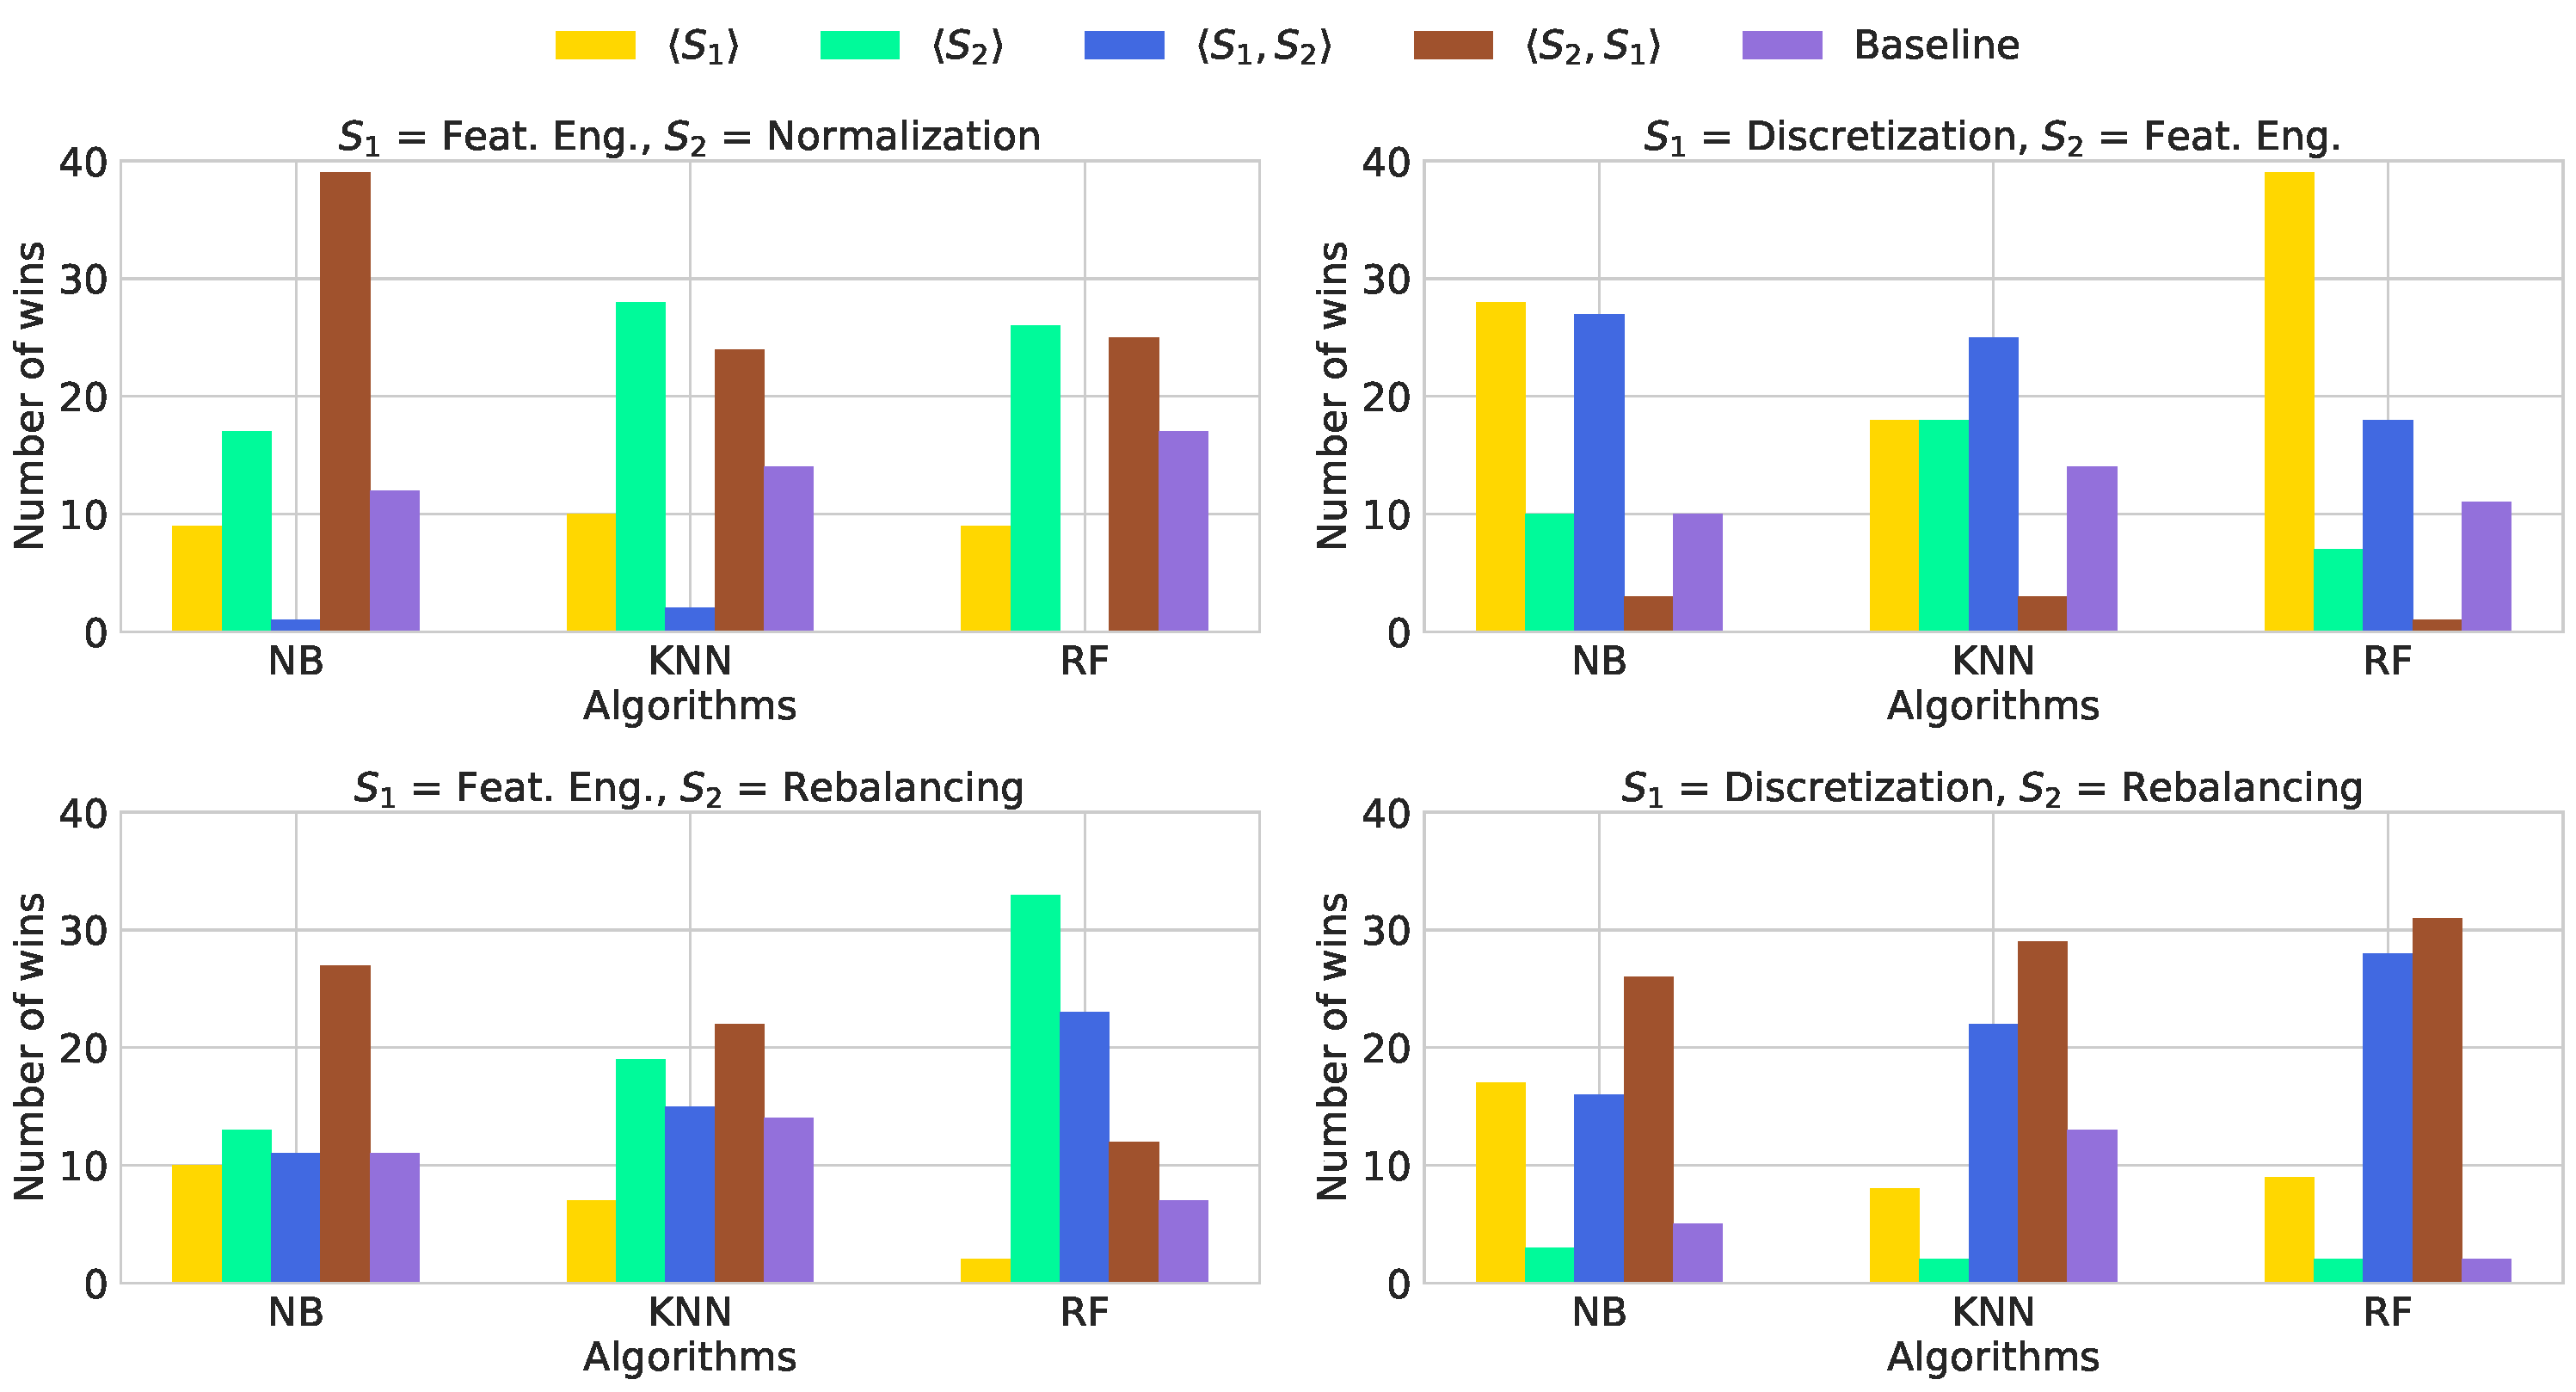
\includegraphics[width=1.0\textwidth]{chapters/data-centric/supervised/img/experiments_results.pdf}
	\caption{Number of datasets for which a given pipeline prototype is declared the winner.}
	\label{effective-fig:learned-rules-results}
\end{figure*}

Applying \Cref{effective-alg:learned-rules}, we obtain a promising order for each pair of transformations considered (i.e., $\{F,N\}$, $\{F,D\}$, $\{F,R\}$, $\{R,D\}$).
Since SMBO is a randomized algorithm, we experimented it with (i) running it several times splitting the budget, and (ii) running it only once with the entire budget.
For the experiments considered, no significant differences where observed, therefore we opted for running it once with the entire budget (i.e., 200 seconds per run), which allows for more configurations to be visited in a single run. Aggregating all the results, \Cref{effective-fig:learned-rules-results} shows the number of datasets, for which a given prototype (\Cref{effective-tbl:validation-rules}, column \textit{winner prototype} for the list of labels) is selected as the winner.
For instance, for the pair $\{F,N\}$ (i.e., Feature Engineering, Normalization), the prototype winning in more datasets for \textit{KNN} and \textit{NB} is $\langle N, F \rangle$.
This means that in general, better results are obtained if Normalization is applied before Feature Engineering.

Next, only $N$ appears as first for \textit{RF} and second best for \textit{KNN} and \textit{NB}, which means that for many datasets, considering different algorithms, it results better to apply only Normalization without combining it with Feature Engineering.
The third position is for $\langle \varnothing, \varnothing \rangle$, which means that for some datasets it is better not to apply any of the steps (in any combination).
The remaining prototypes winning in some datasets are $F$ (only Feature Engineering), and $\langle F, N \rangle$ (Feature Engineering preceding Normalization).
Finally, for three datasets, that are omitted from the figure, there were no winning pipelines (i.e., pipelines resulted in a draw).

Since our goal is to find the best order for a pair of pre-processing steps, we focus on the performances of the pipelines where both of the steps are instantiated (i.e., $\langle S_1, S_2 \rangle$ versus $\langle S_2, S_1 \rangle$).
To do this, we check whether the difference between the number of datasets where they each appear to win is statistically significant by running a binomial test assuming a theoretical probability of $0.5$.
The results are shown in \Cref{effective-tbl:significance-test}.
In summary, the results from \Cref{effective-tbl:significance-test} indicate that, with 95\% confidence we can assume that for the pair $\{F, N\}$, $\langle N, F \rangle$ performs better than $\langle F, N \rangle$, hence Normalization should precede Feature Engineering.
On the other hand, for $\{D, F\}$, $\langle D, F \rangle$ performs better than $\langle F, D \rangle$, hence Discretization should precede Feature Engineering.
Finally, for the remaining transformations, $\{F, R\}$ and $\{R, D\}$, a precedence order can not be pre-assumed since the results obtained are not significant.
Using these results, we create the \textit{Promising precedence} adjacency matrix shown in \Cref{effective-tbl:rules}c, where as one can observe, precedence edges are introduced for $\{N, F\}$ and $\{D, F\}$, but no edges exist neither for $\{F, R\}$, nor for $\{R, D\}$.




\begin{table}[t]
	\centering
	\footnotesize
	\begin{threeparttable}
		\caption{
			Binomial test for determining the order between pairs of transformations. 
		}
		\label{effective-tbl:significance-test}
		\begin{tabular}{@{}cccccc@{}}
			\toprule
			%$S_1$ & $S_2$ & $S_1 \rightarrow S_2$ & $S_2 \rightarrow S_1$ & alpha & \begin{tabular}[c]{@{}c@{}}p-value\\ $H_0:\pi = \pi_0=0.8$\end{tabular} \\ \midrule
			$S_1$ & $S_2$ & $\langle S_1, S_2 \rangle$ & $\langle S_2, S_1 \rangle$ & alpha & p-value\\ \midrule
			$F$ & $N$ & 3 & 88 & 0.05 &  \textbf{0} \\
			$D$ & $F$ & 70 & 7 & 0.05 &  \textbf{0}  \\
			$F$ & $R$ & 49 & 61 & 0.05 & 8.53e-01 \\
			$D$ & $R$ & 66 & 86 & 0.05 & 9.38e-01 \\ \bottomrule
		\end{tabular}
		\begin{tablenotes}
		\centering
		\scriptsize
		\item$N$ - Normalization; $D$ - Discretization; $R$ - Rebalancing; $F$ - Feature Engineering. 
		\end{tablenotes}
	\end{threeparttable}
\end{table}
% \color{black}


\subsubsection{Cross-validation with Chi-square Test}
\label{sec:learned-rules-validation}
After running \Cref{effective-alg:learned-rules} to empirically find a winner between two pairs of transformations, we may obtain a different distribution of the number of wins for the pairs, depending on the datasets considered.
To show that the results obtained with the initial set of datasets are generalizable, we propose to perform an additional cross-validated experiment, where the set of datasets considered can be randomly split into many folds.
Then, for each fold, the results can be compared to the rest, with the aim of checking whether the distributions are similar.
This check can be done via a significance test (e.g., chi-square).
To this end, if the distributions between the folds are similar, it means that the obtained results are independent of the datasets considered, since no matter the combination of the datasets, the results are the same and thus generalizable.

\paragraph{Use case} To show that the results do not depend on the datasests selected, we re-run the experiments (i.e., 10-times each), but this time splitting the datasets into 4-folds.
The goal is to check if the results of the precedence orders from the different folds (i.e., for each experiment considering a randomly different set of datasets) are similar between them (i.e., follow the same distributions).
To confirm this hypothesis, we perform a chi-square test between the results (precedence orders) obtained in a single fold in comparison to the three remaining folds, hence comparing $25$\% of the datasets to the rest.
In particular, to confirm the hypothesis, we need to find results that accept the null hypothesis of the chi-square test which states that ``there is no significant difference between the distributions''.
To do that, sticking to the $95$\% confidence interval, we need to look for p-values greater than $0.05$.
That is, the higher the p-values, the more we accept the null hypothesis, and the more similar the distributions.
Looking at the p-values we found out that they were all much higher than $0.05$.
Specifically, the scores of the chi-square tests of the folds (one fold compared to the rest) are averaged and, after having repeated this procedure 10 times, instead of using a table we depict the 10 averaged p-values using box-plots in \Cref{effective-fig:10-times-4-cv}.
We conclude that, for both of the rules (i.e.,  $\langle F, N \rangle$ and $\langle F, D \rangle$), the significance test indicates a compliance between the new results (\Cref{effective-fig:10-times-4-cv}) and those illustrated above (\Cref{effective-tbl:significance-test}).

\begin{figure*}[!t]
	\centering
	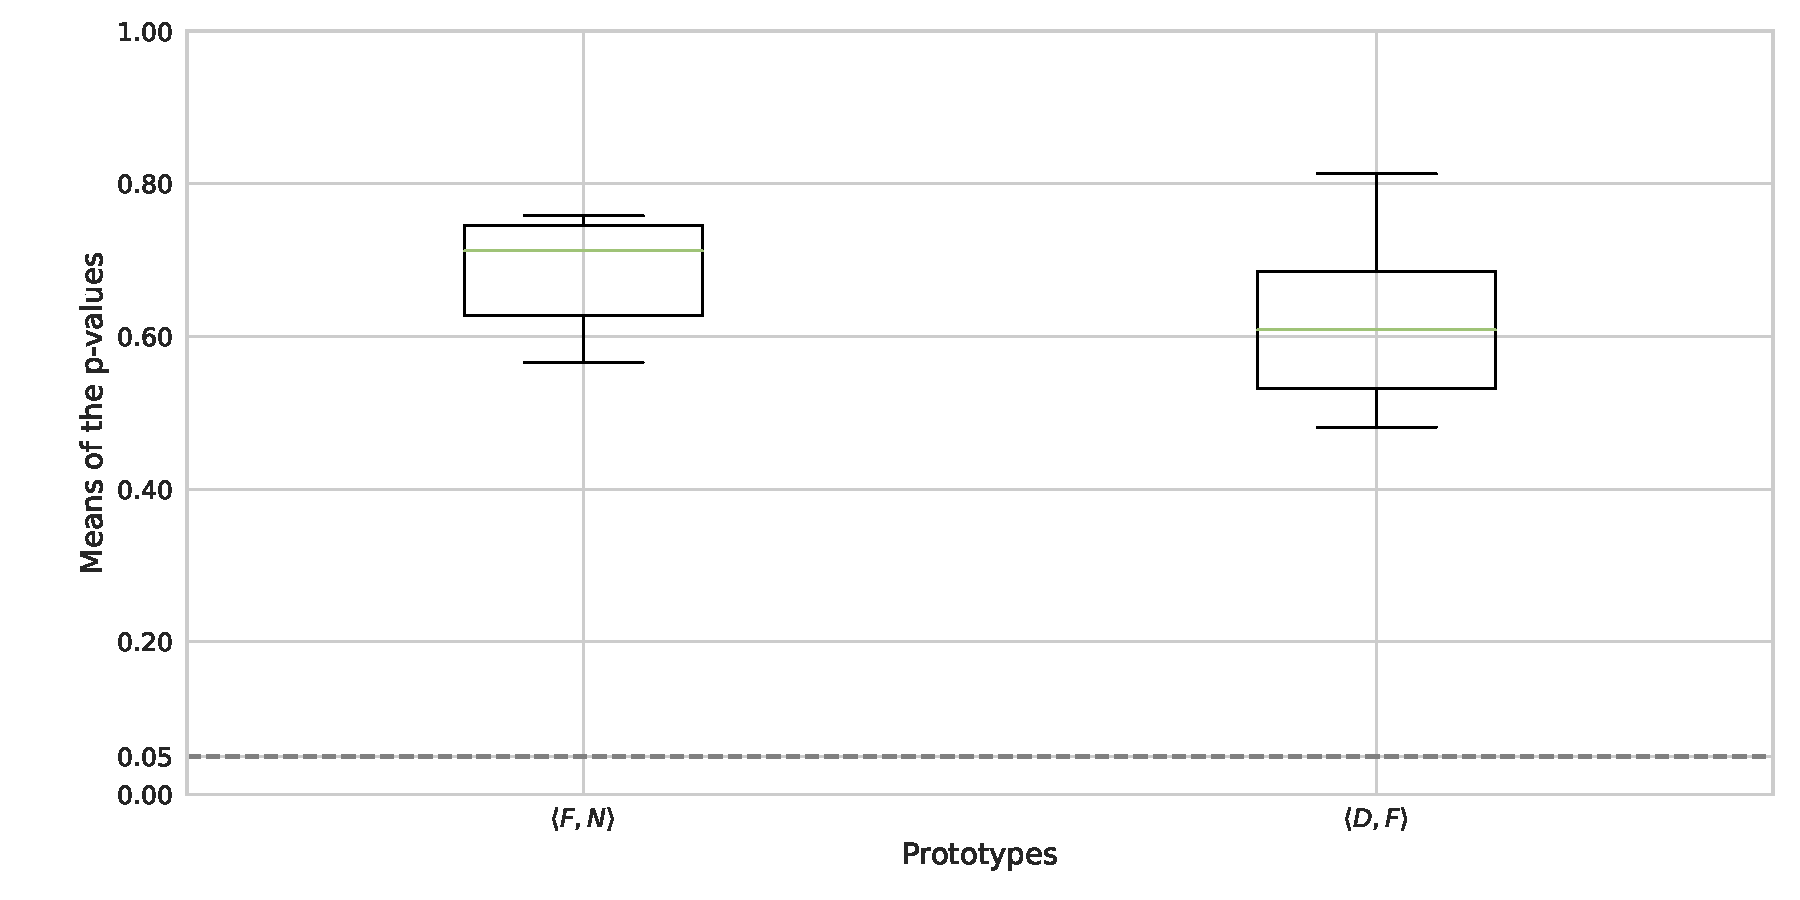
\includegraphics[width=0.9\textwidth]{chapters/data-centric/supervised/img/10_times_4_folds_cv.pdf}
	\caption{The distribution of the p-values obtained after repeating the chi-square test for 10 times, for the 10 times 4-fold cross-validation. \todo{Cambiare la rappresentazione delle pipeline in tutti i grafici}}
	\label{effective-fig:10-times-4-cv}
\end{figure*}

\begin{table}[!t]
	\caption{
		Union of rules from \Cref{effective-tbl:rules}.
	}
	\renewcommand{\arraystretch}{0.3}
	\footnotesize
	\centering
	\label{effective-tbl:rules-union}
	\begin{threeparttable}
		\begin{tabular}{p{1cm}p{1cm}p{1cm}p{1cm}p{1cm}p{1cm}p{1cm}}
			\toprule
			& $\boldsymbol{E}$ & $\boldsymbol{N}$ & $\boldsymbol{D}$ & $\boldsymbol{I}$ & $\boldsymbol{R}$ & $\boldsymbol{F}$
			\\	\cmidrule[.1em]{1-7}
			$\boldsymbol{E}$ & \cellcolor{gray!25} & \texttt{1} & \texttt{1} & \texttt{0} & \texttt{1} & \texttt{1} \\	\cmidrule[.1em]{1-7}
			$\boldsymbol{N}$ & \texttt{0} & \cellcolor{gray!25}  & \texttt{X} & \texttt{0} & \texttt{1} & \texttt{1} \\	\cmidrule[.1em]{1-7}
			$\boldsymbol{D}$ & \texttt{0} & \texttt{X} & \cellcolor{gray!25} & \texttt{0} & \texttt{0} & \texttt{1} \\	\cmidrule[.1em]{1-7}
			$\boldsymbol{I}$ & \texttt{1} & \texttt{1} & \texttt{1} & \cellcolor{gray!25}  & \texttt{1} & \texttt{1} \\	\cmidrule[.1em]{1-7}
			$\boldsymbol{R}$ & \texttt{0} & \texttt{0} & \texttt{0} & \texttt{0} & \cellcolor{gray!25}  & \texttt{0} \\	\cmidrule[.1em]{1-7}
			$\boldsymbol{F}$ & \texttt{0} & \texttt{0} & \texttt{0} & \texttt{0} & \texttt{0} & \cellcolor{gray!25} \\	\cmidrule[.1em]{1-7}
		\end{tabular}
		\begin{tablenotes}
			\scriptsize
			\item$\boldsymbol{E}$ - Encoding; $\boldsymbol{N}$ - Normalization; $\boldsymbol{D}$ - Discretization; $\boldsymbol{I}$ - Imputation; $\boldsymbol{R}$ - Rebalancing; $\boldsymbol{F}$ - Feature Engineering. \item \texttt{1} - a precedence edge exists between the row and the column, \texttt{0} - a precedence edge does not exist between the row and the column, \texttt{X} - the combination is meaningless.
		\end{tablenotes}
	\end{threeparttable}
\end{table}

\subsection{Effective Prototypes Composition}
\label{effective-ssec:composition}

In this, we foresee the composition of the previously defined rules (i.e., for the pairs of pre-processing steps), to generate the final set of rules that would allow to compose longer chains---consisting of more than two steps.
This is when we also resolve the inconsistencies and define precedences for the pairs of steps that may not have any precedence defined already---in that case, we basically take into account all the permutations.
This allows to finally generate the possible effective  prototypes.

\paragraph{Use case}
To generate the final prototypes, in this phase, we combine all the matrices generated by the previous steps.
That is, we take the union of the edges (represented by \texttt{1}'s) from the matrices in \Cref{effective-tbl:rules} (a,b,c), and create a new final adjacency matrix, shown in \Cref{effective-tbl:rules-union}.
This is the matrix that will allow us to generate the final effective prototypes.

Observing the table, one can realize that for pairs $\{F,R\}$ and $\{R,D\}$, no precedence edges exist.
This means that these pairs are somewhat equally relevant from either direction (any order), and thus when generating the final prototypes, both options should appear.

For a better reading, in Figure~3.6, we visualize \Cref{effective-tbl:rules-union} in form of a graph, where nodes represent the pre-processing steps and the directed edges represent a precedence order between them.
Out of the graph, we generate the final prototypes by taking all the maximum length variations (ordered arrangements without repetition) of the nodes, respecting the precedence rules (i.e., not contradicting the direction of existing edges).
The result is the set of five prototypes shown in Table 3.7. This set consisting of \textit{compatible}, \textit{meaningful} and \textit{promising} pairs of transformations is the set of recommended \textit{effective pipeline prototypes}.


\begin{figure}
	\begin{floatrow}
	\ffigbox{
		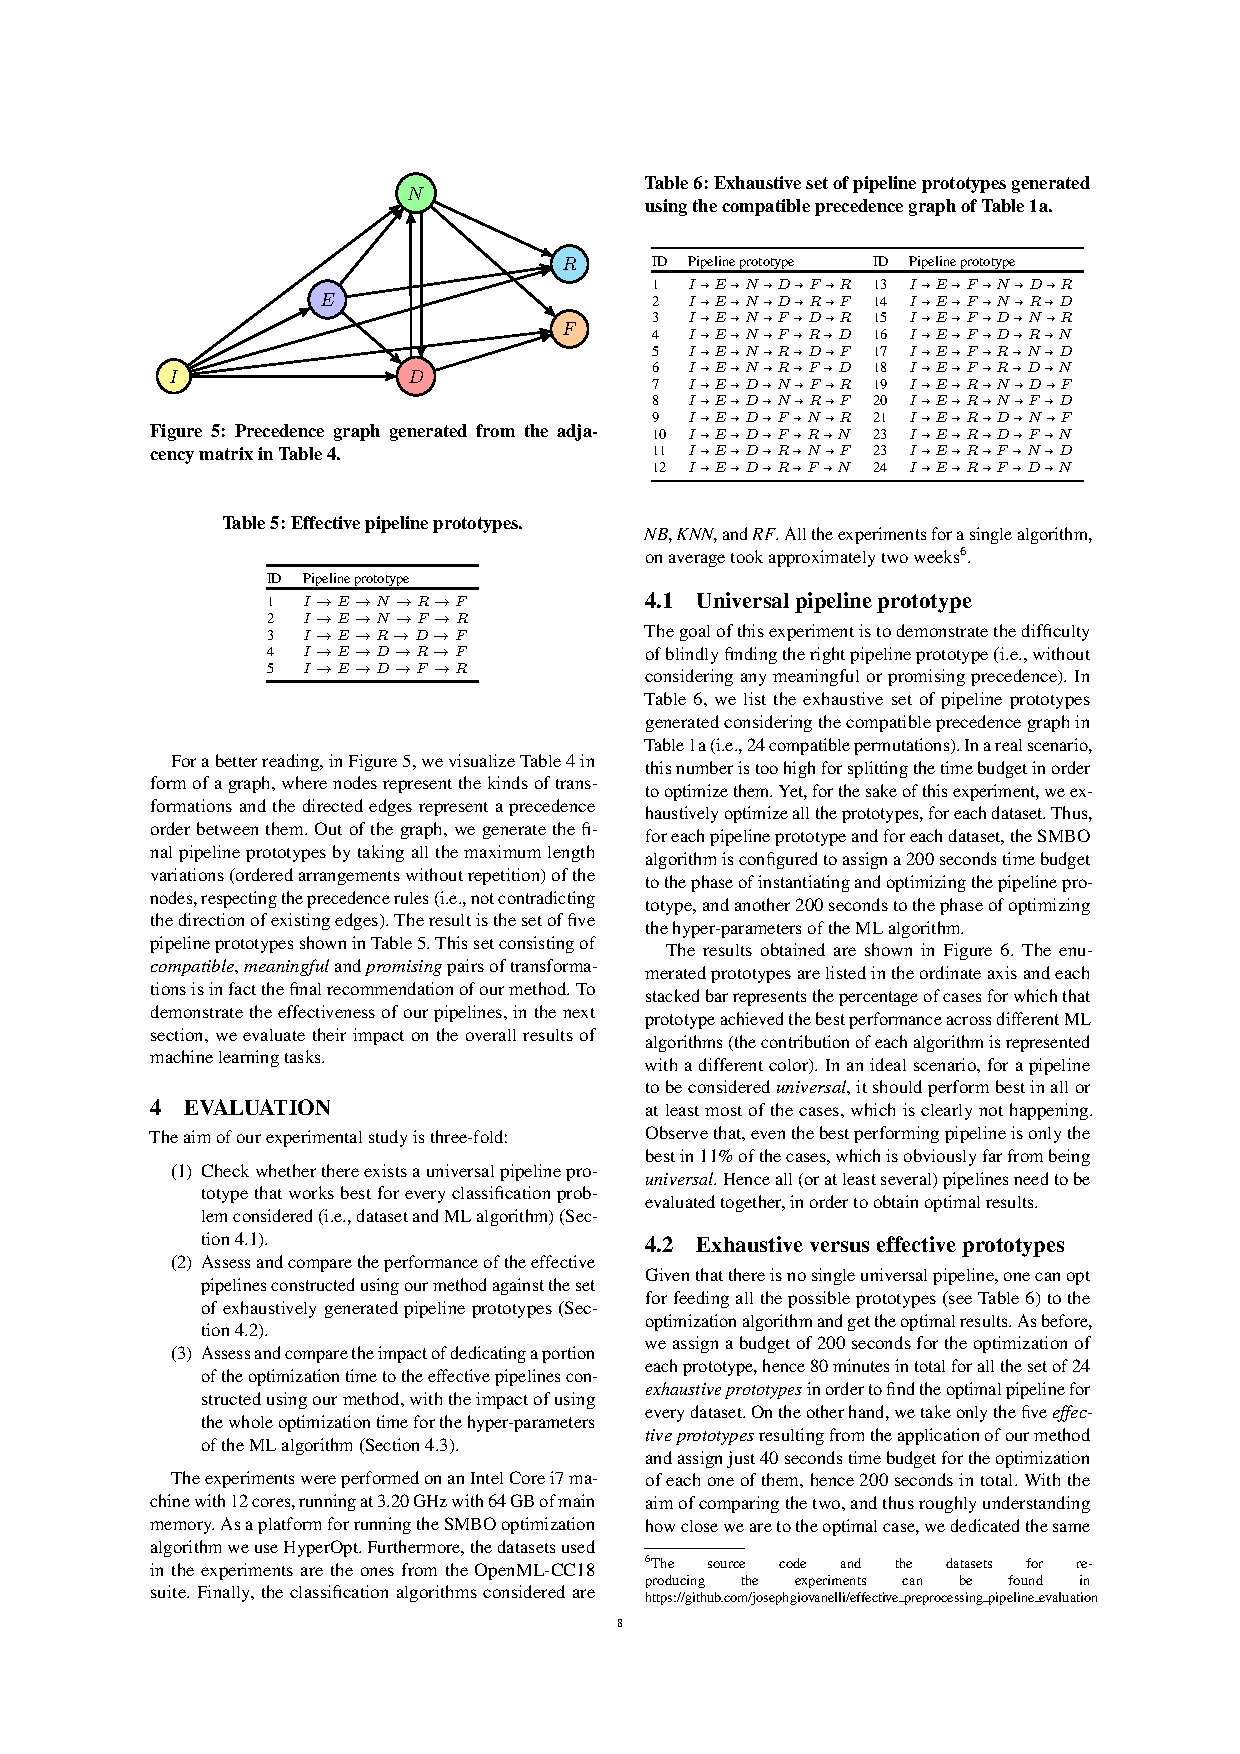
\includegraphics[clip, trim=2.5cm 23cm 10.5cm 2cm,width=0.5\textwidth]{chapters/data-centric/supervised/img/graph.pdf}
	}{
		  \caption{Precedence graph generated from \Cref{effective-tbl:rules-union}.}
	}
	\capbtabbox{
	\begin{tabular}{@{}ll}
				\toprule
				ID& Pipeline prototype                                             \\ \toprule
				1&{\color[HTML]{000000} $\langle I, E, N, R, F  \rangle$} \\
				2&{\color[HTML]{000000} $\langle I, E, N, F, R \rangle$} \\
				3&{\color[HTML]{000000} $\langle I, E, R, D, F \rangle$} \\
				4&{\color[HTML]{000000} $\langle I, E, D, R, F \rangle$} \\
				5&{\color[HTML]{000000} $\langle I, E, D , F, R \rangle$} \\
				\bottomrule
			\end{tabular}
	}{
		  \caption{Effective prototypes generated from Figure~3.6.
		}
	}
	\end{floatrow}
\end{figure}

\subsection{Meta-learning of Instantiation Rules}
\label{effective-ssec:meta-learning}

Once the pipeline prototypes are constructed (i.e., the order between the steps is defined), what follows is their instantiation with the actual transformations.
For that, one can rely completely on SMBO, and let the optimization choose the right transformation for each step.
However, as many optimization techniques, SMBO suffers from the cold-start problem where, in the beginning, it does not have enough information to come up with promising configurations, and a wrong choice may affect the whole process.

\subsubsection{Exploratory Analysis}
Given the availability of the experimental SMBO executions (executed in an exhaustive manner, considering all the prototypes), one can perform an exploratory analysis with the aim of removing useless prototypes, executable pipelines or sngle transformations.
Hence, further tweaking the search space.
In particular, one might analyze whether:

\begin{itemize}
    \item there exist some combination of steps (\Cref{effective-tbl:pipeline-enumeration}), that are generally useless (i.e., in terms of their impact on the final performance), and thus can be discarded a priori to reduce the search space;
    \item there are some executable pipelines that are consistently chosen more often than others by the optimization, meaning that they are more useful than others;
    \item within the executable pipelines, some transformations are chosen more often than others, meaning that they provide a more positive impact.
    \end{itemize}

\paragraph{Use case}
We performed the above-mentioned analysis, but this did not lead to any conclusive or significant results.
In particular, as shown in \Cref{effective-fig:prototypes-impact}, we could not find any useless prototypes---not positively impacting the final accuracy, that could be discarded a priori from the potential list of prototypes.
Actually, as we will show in \Cref{effective-sec:eval-universal-pipeline}, all of them lead to the best in one case or another, which does not mean the epsilon improvement some provide is worth the search cost you incur in considering them (but this more in-depth analysis is done later).
Next, as shown in \Cref{effective-fig:pipeline-frequency}, there were no physical pipelines shown to be more useful---hence more often selected, than others.
Even if $\langle N , R \rangle$ is clearly above, it barely reaches 30\% in KNN.
Finally, observing \Cref{effective-fig:transformation-frequency}, it is clear that some kinds of transformations are chosen more often, but looking closely (i.e., the shaded bars), it is not clear which operator brings more benefit.
For instance, Normalization is present in 90\% of the pipelines, but it is not easy to distinguish which kind of Normalization (i.e., actual operator) is more beneficial.
For this, we need more complex rules or guidelines that may help in finding the right operator to use.


\begin{figure*}[!t]
	\centering
	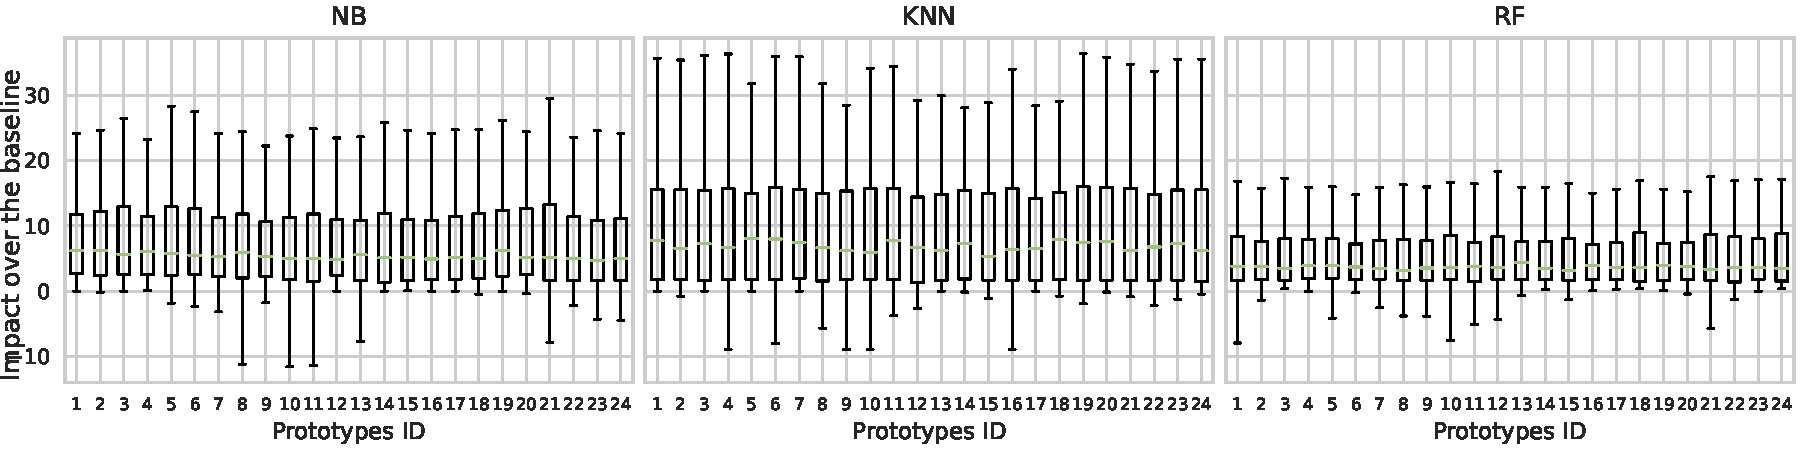
\includegraphics[width=1.0\textwidth]{chapters/data-centric/supervised/img/prototypes_impact.pdf}
	\caption{The impact of the different pipeline prototypes over the baseline (i.e., when no transformation is applied).}
	\label{effective-fig:prototypes-impact}
\end{figure*}

\begin{figure*}[!h]
	\centering
	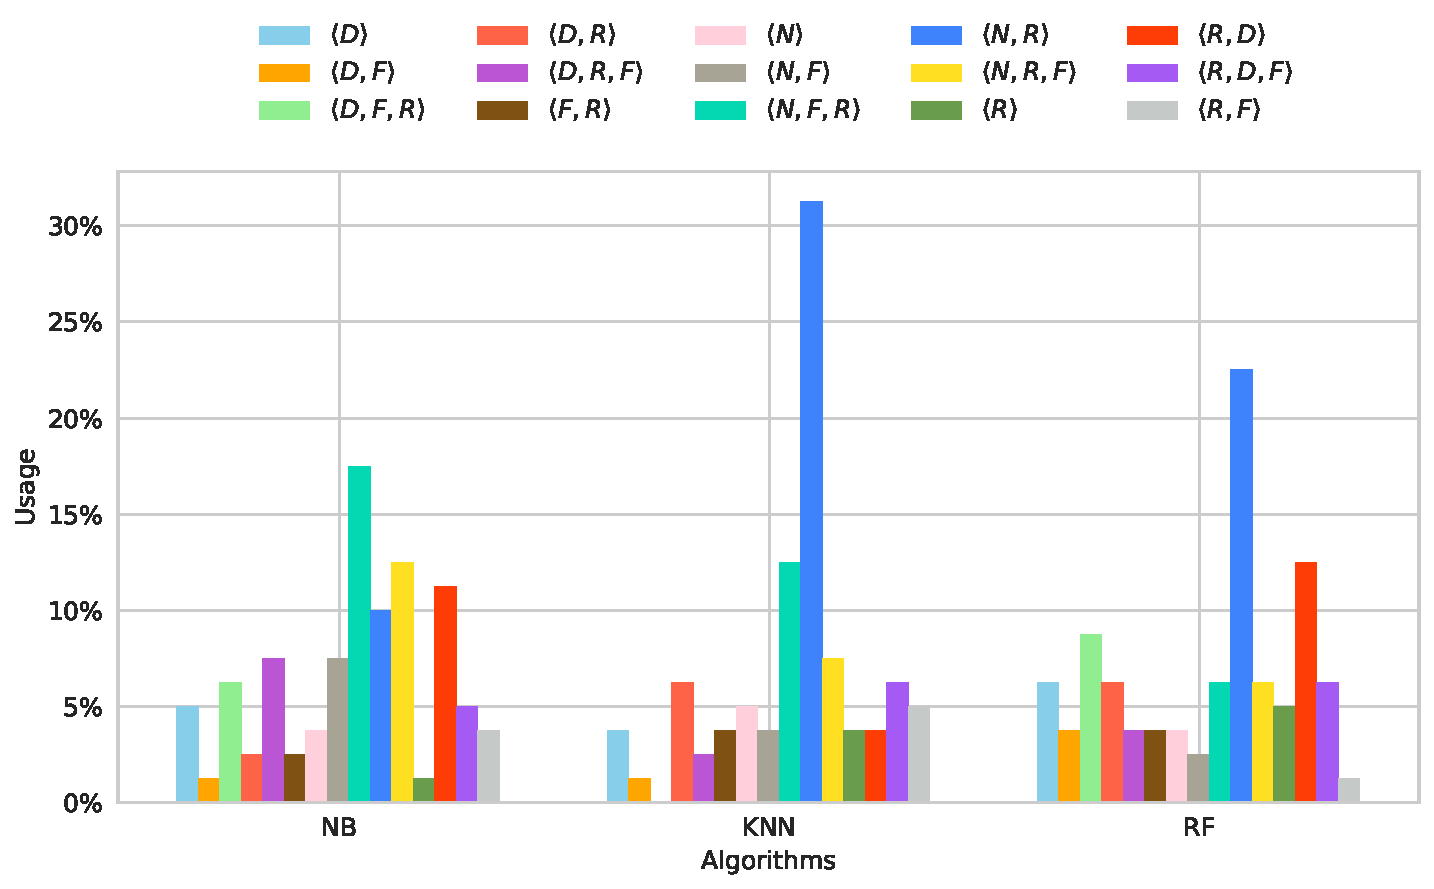
\includegraphics[width=1.0\textwidth]{chapters/data-centric/supervised/img/pp_pipeline_study2.pdf}
	\caption{Percentage of use of the different physical pipelines.}
	\label{effective-fig:pipeline-frequency}
\end{figure*}

\begin{figure*}[!h]
	\centering
	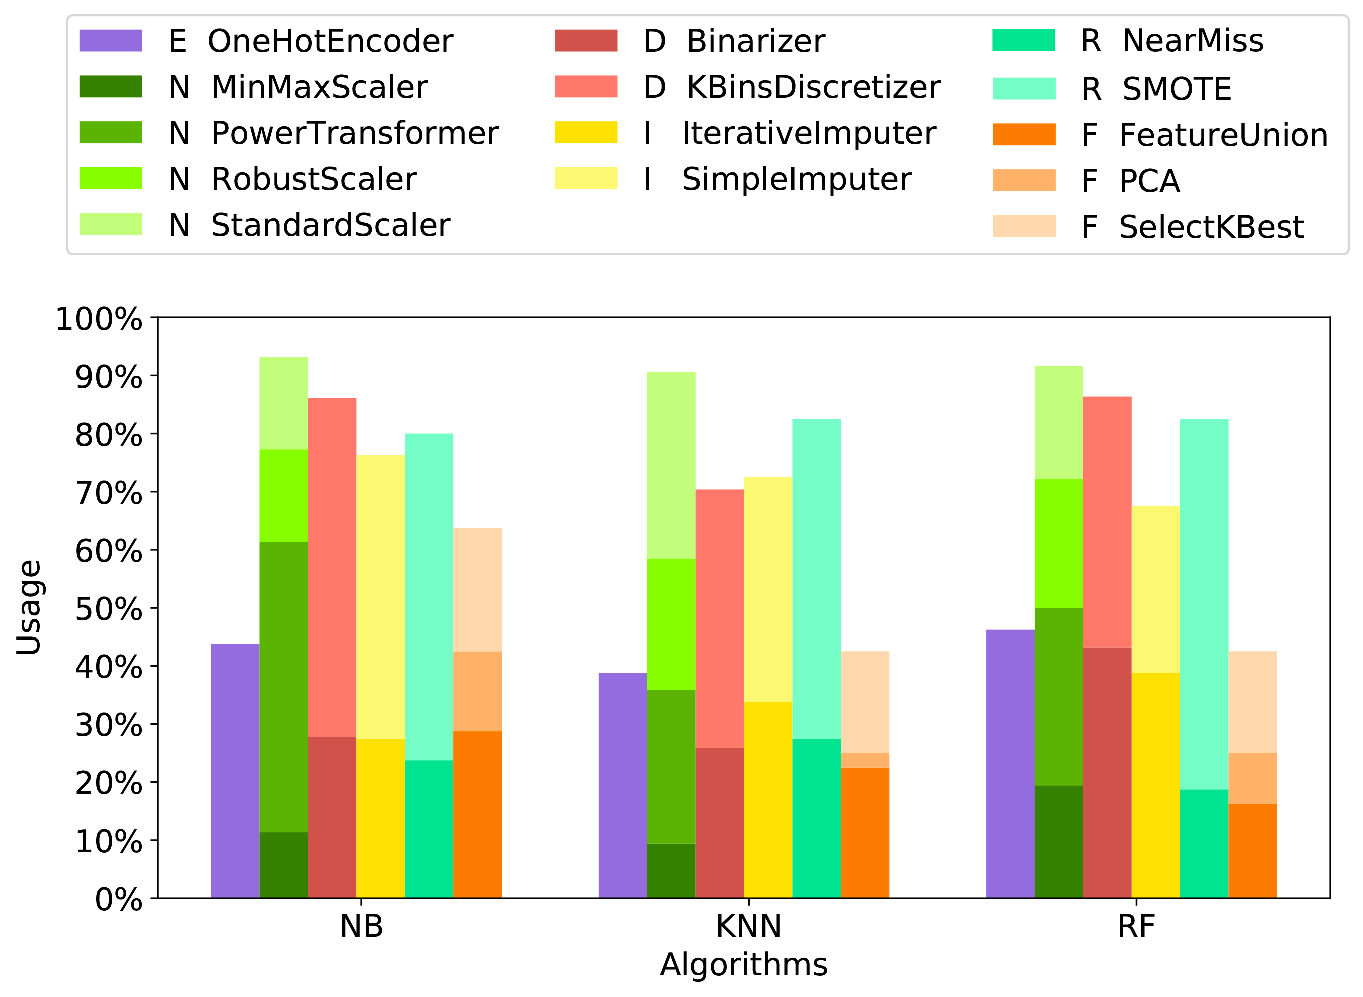
\includegraphics[width=0.7\textwidth]{chapters/data-centric/supervised/img/pp_pipeline_study_grouped.pdf}
	\caption{Percentage of use of a transformation in a physical pipeline.}
	\label{effective-fig:transformation-frequency}
\end{figure*}

\subsubsection{Meta-learning}
To mitigate the cold-start problem, we propose to perform meta-learning, where we intend to use the knowledge extracted from historical data in order to devise rules that may help the optimization in its initial settings.
Meta-learning is the process of ``learning on top of learning'', or learning a model using historical data from ML experiments.
Traditionally, it has been used for predicting the performance (e.g., accuracy) of an algorithm on a given dataset.
That is, given some historical runs of the performance of classification algorithms over various datasets (i.e., meta-dataset: consisting of datasets characteristics as meta-features and the performance of the ML algorithm as the desired outcome in a regression task), one can learn a model (i.e., meta-model), that is able to predict the performance of a given ML algorithm on a new dataset \cite{Brazdil04Book}.
Lately, this technique has been extended in order to predict the impact of pre-processing steps over the performance of ML algorithms and thus rank them based on the impact \cite{Bilalli17AMCS, presistant18CSI, presistant19DKE}.
The same idea can be applied to learning the best trnasformation for a given step.
That is, through meta-learning one can learn the intrinsic relationship between dataset characteristics and the transformation performance, and thus come up with rules that are not obvious and are effective at the time of pipeline instantiation.
The main idea is to build a model, that is able to predict the transformation for a certain pre-processing step, given the meta-features extracted from the dataset considered for the optimization.
This translates to answering the following question: ``given that we know the dataset characteristics and having selected a certain pre-processing step (e.g., Imputation), what is the optimal transformation we need to obtain the highest improvement w.r.t. loss (i.e., when the ML algorithm is applied over the transformed dataset)?''.
In particular, the model can generate a set of complementary rules that help in the optimization, providing a good starting instantiation for some of the steps in the prototype.

To train the model we need a meta-dataset that can be  (i) generated through optimization algorithms (e.g., SMBO executions), (ii) generated manually through simple evaluations of classification algorithms over transformed datasets, or (iii) assumed already given (e.g., OpenML).
Given a meta-dataset, we propose to learn to predict the best instantiation (transformation) for a given pre-processing step, including skipping the step (class \texttt{None}).

\paragraph{Use case}
Our training dataset for the meta-learning (i.e., meta-dataset) is built through SMBO runs on the OpenML datasets (\Cref{effective-ssec:rules-learned}).
We first extract the dataset characteristics (i.e., meta-features; e.g., number of features, number of instances, number of missing values).
Then, by applying SMBO optimization on classification algorithms and pre-processing prototypes, for each dataset, we retrieve the loss (in our case, accuracy) of the ML algorithms over the optimized pipelines.
This gives us the optimized executable pipelines and their impact on the accuracy of the learning algorithms for each dataset at hand.
Given such information, our aim is to now save time and improve the instantiation of the transformations for each step considered in the prototype.

We trained several different conditional inference trees (i.e., a particular implementation of decision trees \cite{ctree}) because they produce models that can be easily read and interpreted.
Specifically, the independence of each meta-feature with the class (transformation of a specific step) is tested through a statistical test.
The split is made on the variable with the lowest p-value.
We report the p-value too so that it can be seen how strong the association is (i.e., why that variable was chosen).
We stick with the p-value threshold of $0.05$, and devise a rule from any branch of the tree that is within the threshold.
In the following, we describe the rules obtained within the selected significance threshold.


\begin{figure}[!h]
	\centering
	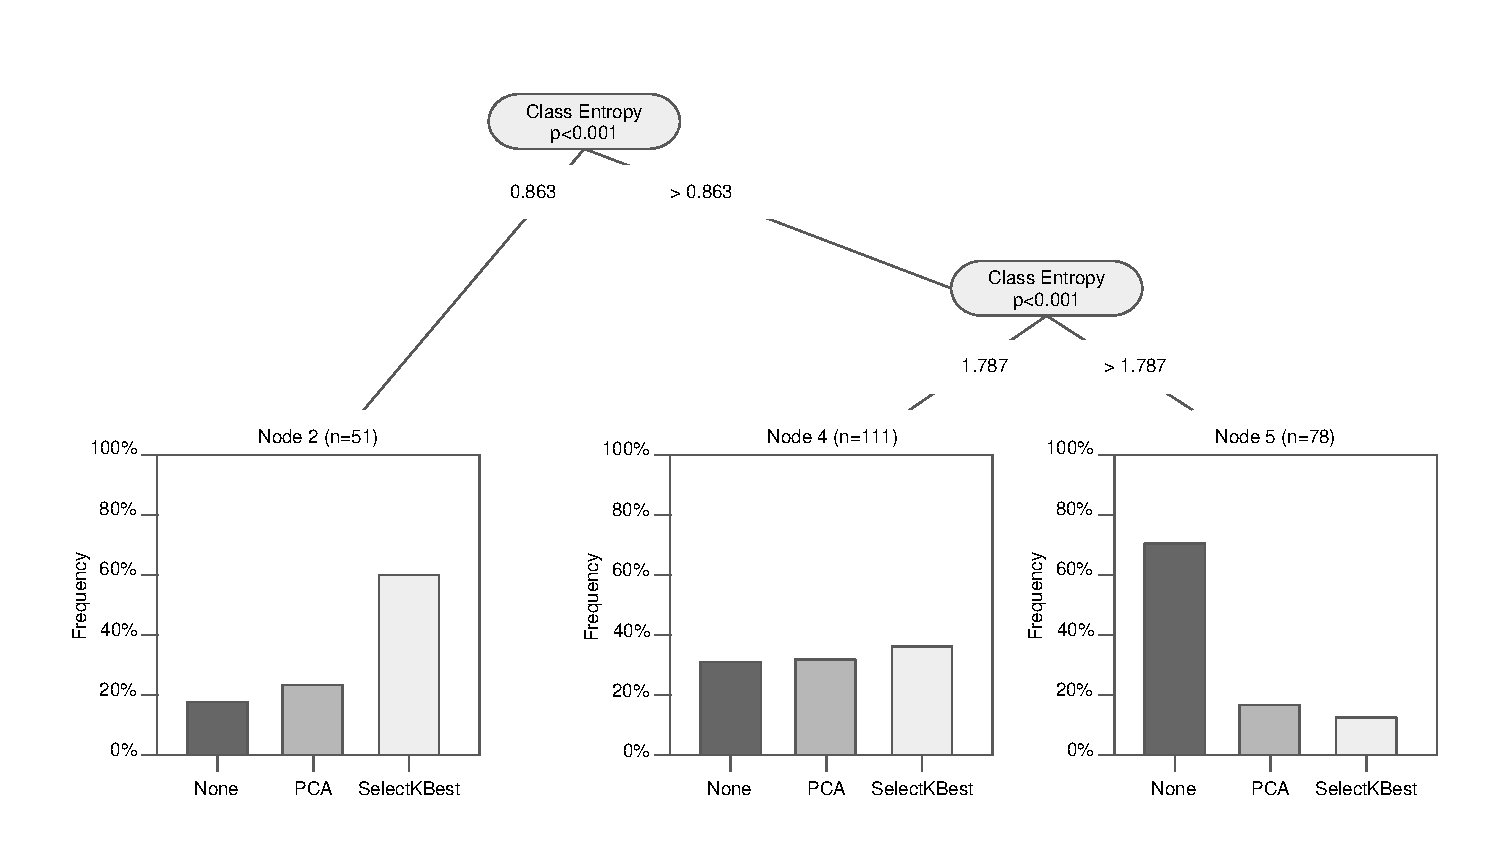
\includegraphics[clip, trim=1.0cm 0.4cm 1cm 1cm,width=1\textwidth]{chapters/data-centric/supervised/img/tree-FE.pdf}
	\caption{Conditional Inference Tree built for the \textit{Features Engineering} transformation.}
	\label{effective-fig:features-meta-learning:feature-engineering}
\end{figure}

\textbf{Rules for Feature Engineering}. The available transformations in scikit-learn for Feature Engineering are: Principal Component Analysis (\texttt{PCA}), \texttt{Feature Selection} (Select K Best), \texttt{Both} (PCA + Select K Best), and \texttt{None}.
The tree generated for the Feature Engineering transformation is shown in \Cref{effective-fig:features-meta-learning:feature-engineering}.
The leaves show the selected transformation frequency.
For the sake of simplicity, we do not consider the union of PCA and Select K Best as a transformation per se, instead we distribute that contribution to the two operators that compose it.
Observe that there is a strong correlation between the Feature Engineering transformation and the entropy of the class.
Indeed, such a meta-feature achieved a p-value smaller than $0.001$.
We can clearly read that if the Class Entropy is low, then \texttt{Feature Selection} is way more chosen than the other options (see Node 2).
Recall that entropy is a measure of how much disorder there is in its domain.
The less is that value, the easier is the classification problem.
As a consequence, it is reasonable to think that the easier the classification problem is, the more likely is the fact that the class can be described by a low number of features.
Hence, the \texttt{Feature Selection} technique can be successfully applied.
Conversely, Node 5 shows that, when the Class Entropy is high, it is better to not apply any Feature Engineering operator.
As a matter of fact, a high value of Class Entropy involves a high number of classes and/or few instances per class, hence a really difficult problem.
In such cases, reducing the dimensionality of the dataset does not lead to any improvement.
Finally, when the Class Entropy is in between, there is no clear winner, and thus other non-obvious factors may affect the choice of the operator.

\begin{figure}[!h]
	\centering
	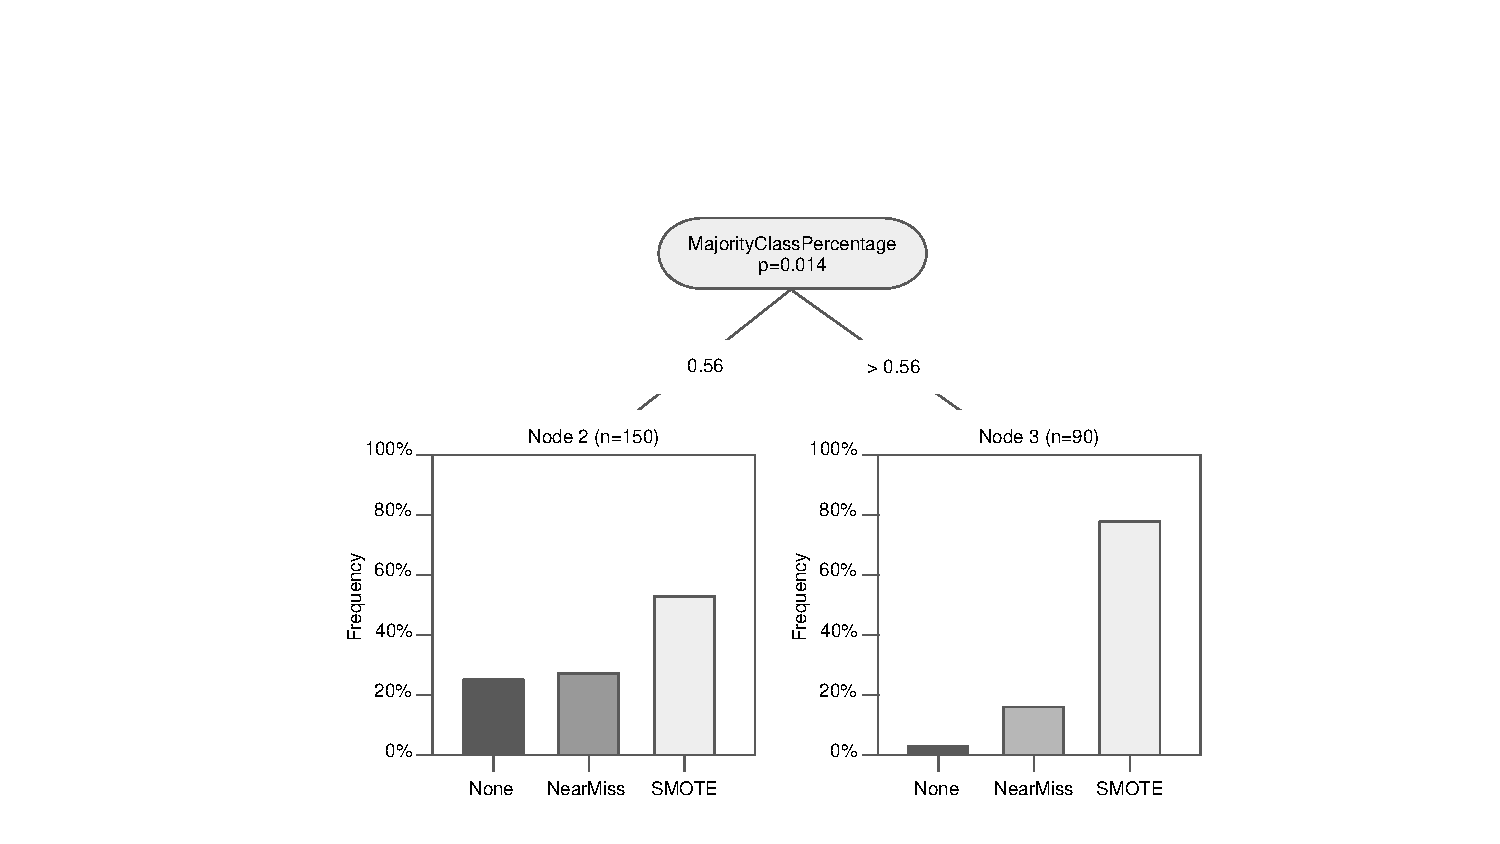
\includegraphics[clip, trim=5.8cm 0.4cm 5.05cm 3.5cm,width=0.65\textwidth]{chapters/data-centric/supervised/img/tree-RE.pdf}
	\caption{Conditional Inference Tree built for the \textit{Rebalancing} transformation.}
	\label{effective-fig:features-meta-learning:rebalancing}
\end{figure}

\textbf{Rules for Rebalancing}. As for Rebalancing, the transformations considered from the imblearn\footnote{\url{https://pypi.org/project/imbalanced-learn}} library are: \texttt{Near Miss}, \texttt{SMOTE}, and \texttt{None}.
The first is an undersampling algorithm which randomly eliminates the samples from the larger class; the second is an oversampling technique that creates samples of the minority class, as a linear combination of them.
As shown in \Cref{effective-fig:features-meta-learning:rebalancing}, the meta-feature Majority Class Percentage has a p-value of $0.014$.
This can be read as, in case of an unbalanced class problem (i.e., Node 3: Majority Class Percentage greater than 56), an oversampling of the minority class(es) is preferred to a downsampling of the majority one(s).
However, when the Majority Class Percentage is smaller than 56\%, the situation is not that clear, and there is no technique that is applied significantly more often than the rest; they are close to each other.
Therefore, it is difficult to understand which problems (which dataset characteristics do they have) belong to Node 2.
In summary, when the majority class has no more than 56\% , it implies that it is an unbalanced class, and as mentioned above, SMBO tends to choose the same transformation.
However, when the majority class has less than 56\%, it may imply that: (i) there are just two classes and the problem counts as a balanced problem, so no transformation needs to be applied, or (ii) it is a multi-class problem, and thus there is no clear winner in terms of transformation.

\subsection{Data Pipeline Instantiation}
\label{effective-ssec:prototype-insta}

The prototypes from the top flow and the meta-lerning rules from the bottom flow (if the optimization framework permits) are finally fed to the final phase which deals with the instantiation and optimization of the prototypes. In this, we run SMBO until an optimized pipeline is found.

\paragraph{Use case}
 In our final execution, we run SMBO to find a suitable instantiation for the suggested prototypes. The simple but not obvious meta-learning rules, even though not included in our final execution, because of the implementation considered (i.e., HyperOpt), can potentially be used to ease the cold-start problem.

\section{Evaluation}
\label{effective-sec:evaluation}


The aim of our experimental study is three-fold:
\begin{enumerate}
    \item Check whether there exists a universal prototype that works best for any classification problem considered  (i.e., dataset and ML algorithm) (\Cref{effective-sec:eval-universal-pipeline}).
    \item Assess and compare the performance of optimizing the effective prototypes constructed using our method against the set of exhaustively generated prototypes (\Cref{effective-sec:eval-our-vs-rest}).
    \item Assess and compare the impact of dedicating a portion of the optimization time to the effective prototypes against using the whole optimization time for the hyperparameters of the ML algorithm (\Cref{effective-sec:eval-dpso-vs-cash}).
\end{enumerate}

The experiments were performed on an Intel Core i7 machine with 12 cores, running at 3.20 GHz with 64 GB of main memory.
We leveraged the SMBO optimization algorithm available in the Python library HyperOpt \cite{bergstra2015hyperopt}.
The datasets used in the experiments are the ones from the OpenML CC-18 repository \cite{OpenML2013}.
Finally, the classification algorithms considered are \textit{NB}, \textit{KNN}, and \textit{RF} from the Python library Scikit-learn \cite{scikit-learn}.
All the experiments for a single algorithm took approximately two weeks.


\paragraph{AutoPrep}
With the recent shift towards data-centric approaches, rather than algorithmic, data pre-processing is receiving a lot of attention.
Yet, its impact on the final analysis is not widely recognized, primarily due to the lack of publicly available experiments that quantify it.
To bridge this gap, along with this work, we contribute to publishing a companion reproducibility paper \cite{Giovanelli2022IS} for the experiments and results reported in the following.
AutoPrep introduces a set of reproducible experiments on the impact of data pre-processing by providing a detailed reproducibility protocol together with a software tool and a set of extensible datasets, which allow for all the experiments and results of this chapter reproduced.
Our experiments have been performed among different machines with different resources.
We achieved to deploy \textit{strongly reproducible experiments}, when based on a collection of intermediate results, and \textit{weakly reproducible experiments} when reproducing our end-to-end optimization from scratch.
The reproducibility protocol is created in Docker and tested in Windows and Linux.
The source code and the datasets for reproducing the experiments can be found on GitHub\footnote{
\url{https://github.com/josephgiovanelli/autoprep}}.

\begin{definition}[Strongly reproducible experiment  \cite{reproducible}]
    \label{def:strong}
    Given a set of previously reported experimental results and conclusions, a computational experiment is strongly reproducible if it allows to confirm both previously reported results and conclusions exactly.
\end{definition}

\begin{definition}[Weakly reproducible experiment  \cite{reproducible}]
    \label{def:weak}
    Given a set of previously reported experimental results and conclusions, a computational experiment is weakly reproducible if the Spearman rank correlation between the original and reproduced results is equal to 1, and their Pearson correlation value is high enough to allow the confirmation of all previously reported conclusions, even if the reproduced results do not reproduce all results exactly. Thus, weak reproducibility is a performance-rank-preserving notion.
\end{definition}

\subsection{Universal Pipeline Prototype}
\label{effective-sec:eval-universal-pipeline}
The goal of this experiment is to demonstrate the difficulty of blindly finding the right prototype (i.e., without considering any meaningful or promising precedence).
In \Cref{effective-tbl:pipeline-enumeration}, we list the exhaustive set of pipeline prototypes generated considering the compatible precedence graph in Table~\ref{effective-tbl:rules}a (i.e., 24 compatible permutations).
In a real scenario, this number would be too high for splitting the time budget in order to optimize them.
Yet, for the sake of this experiment, we exhaustively optimize all the prototypes, for each dataset.
Thus, for each prototype and for each dataset, the SMBO algorithm is configured to assign a 200 seconds time budget to the phase of instantiating and optimizing the prototype, and another 200 seconds to the phase of optimizing the hyperparameters of the ML algorithm.

\begin{table}[t]
\caption[Enumeration of the prototypes that can be generated by compatible precedence]{Exhaustive set of prototypes generated using the compatible precedence graph of Table~\ref{effective-tbl:rules}a. $E$ - Encoding; $N$ - Normalization; $D$ - Discretization; $I$ - Imputation; $R$ - Rebalancing; $F$ - Feature Engineering.
}
\footnotesize
\label{effective-tbl:pipeline-enumeration}
\begin{center}
\begin{tabular}{@{}lllll@{}}
\toprule
ID & Pipeline prototype & ID & Pipeline prototype                                                                   \\ \toprule
1  & {\color[HTML]{000000} $\langle I, E, N, D, F, R \rangle$} & 13 & {\color[HTML]{000000} $\langle I, E, F, N, D, R \rangle$} \\
2  & {\color[HTML]{000000} $\langle I, E, N, D, R, F \rangle$} & 14 & {\color[HTML]{000000} $\langle I, E, F, N, R, D \rangle$} \\
3  & {\color[HTML]{000000} $\langle I, E, N, F, D, R \rangle$} & 15 & {\color[HTML]{000000} $\langle I, E, F, D, N, R \rangle$} \\
4  & {\color[HTML]{000000} $\langle I, E, N, F, R, D \rangle$} & 16 & {\color[HTML]{000000} $\langle I, E, F, D, R, N \rangle$} \\
5  & {\color[HTML]{000000} $\langle I, E, N, R, D, F \rangle$} & 17 & {\color[HTML]{000000} $\langle I, E, F, R, N, D \rangle$} \\
6  & {\color[HTML]{000000} $\langle I, E, N, R, F, D \rangle$} & 18 & {\color[HTML]{000000} $\langle I, E, F, R, D, N \rangle$} \\
7  & {\color[HTML]{000000} $\langle I, E, D, N, F, R \rangle$} & 19 & {\color[HTML]{000000} $\langle I, E, R, N, D, F \rangle$} \\
8  & {\color[HTML]{000000} $\langle I, E, D, N, R, F \rangle$} & 20 & {\color[HTML]{000000} $\langle I, E, R, N, F, D \rangle$} \\
9  & {\color[HTML]{000000} $\langle I, E, D, F, N, R \rangle$} & 21 & {\color[HTML]{000000} $\langle I, E, R, D, N, F \rangle$} \\
10 & {\color[HTML]{000000} $\langle I, E, D, F, R, N \rangle$} & 23 & {\color[HTML]{000000} $\langle I, E, R, D, F, N \rangle$} \\
11 & {\color[HTML]{000000} $\langle I, E, D, R, N, F \rangle$} & 23 & {\color[HTML]{000000} $\langle I, E, R, F, N, D \rangle$} \\
12 & {\color[HTML]{000000} $\langle I, E, D, R, F, N \rangle$} & 24 & {\color[HTML]{000000} $\langle I, E, R, F, D, N \rangle$}
\\ \bottomrule
\end{tabular}
\end{center}
\end{table}

The results obtained are shown in \Cref{effective-fig:eval-universal-pipeline}.
The enumerated prototypes are listed in the abscissa axis and each stacked bar represents the percentage of cases for which that prototype achieved the best performance across different ML algorithms (the contribution of each algorithm is represented with a different color).
In an ideal scenario, for a prototype to be considered \textit{universal}, it should perform best in all or at least most of the cases, which is clearly not happening.
Observe that, even the best-performing prototype is only the best in 19\% of the cases, which is obviously far from being \textit{universal}.
Hence all (or at least several) prototypes need to be evaluated together, in order to obtain better solutions.

\begin{figure}[t]
    \centering
    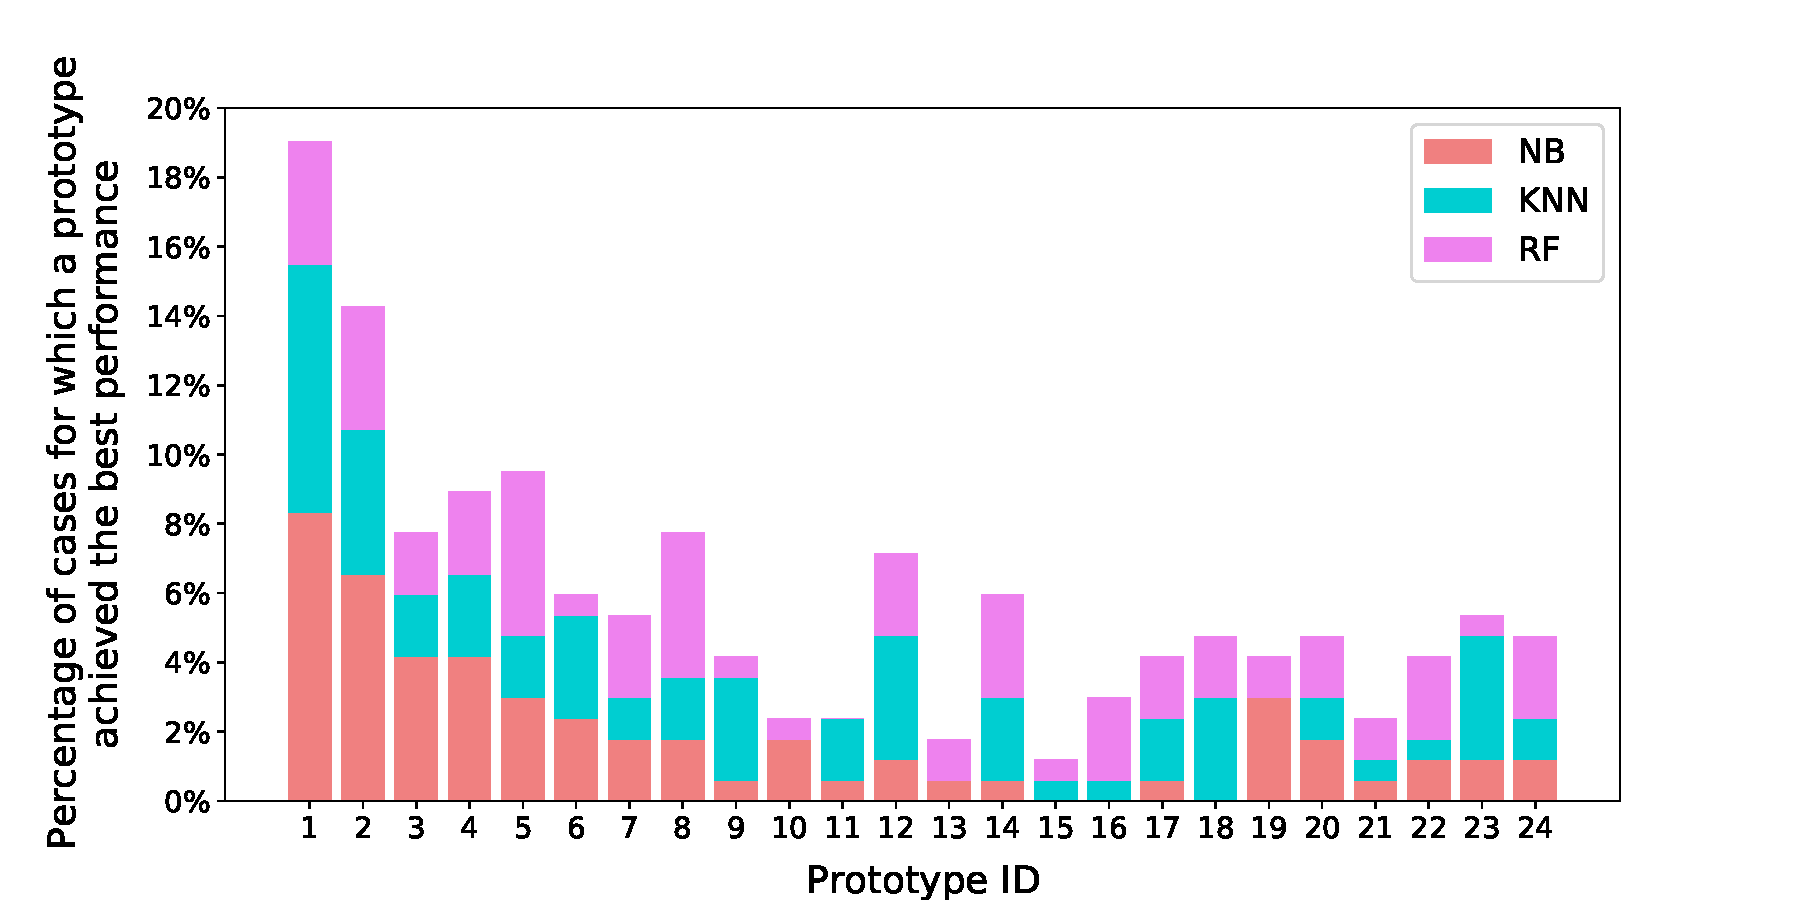
\includegraphics[width=0.8\textwidth]{chapters/data-centric/supervised/img/evaluation1.pdf}
    \caption{Comparison of the goodness of the exhaustive set of prototypes.}
    \label{effective-fig:eval-universal-pipeline}
\end{figure}

\subsection{Exhaustive Versus Effective Prototypes}
\label{effective-sec:eval-our-vs-rest}
Given that there is no single universal prototype, one can opt for feeding all the possible prototypes (see \Cref{effective-tbl:pipeline-enumeration}) to the optimization algorithm in order to get the best solutions out of them.
As before, we assign a budget of 200 seconds for the optimization of each prototype, hence 80 minutes in total for all the set of 24 \textit{exhaustive prototypes} in order to find the optimal pipeline for every dataset.
On the other hand, we take only the five \textit{effective prototypes} resulting from the application of our method and assign just 40 seconds time budget for the optimization of each one of them, hence 200 seconds in total. With the aim of comparing the two, and thus roughly understanding how close we are to the optimal case, in both cases, we dedicated the same time budget (i.e., 200 seconds) for the phase of optimizing the hyperparameters of the ML algorithm.
In order to evaluate how close the \textit{effective prototypes} are to the \textit{exhaustive ones}, we calculate the \textit{normalized distance} from the result to the optimum---w.r.t. accuracy.

\begin{equation*}
    normalized\;distance = \frac{ACC_{\textup{eff}} - ACC_{\varnothing}}{ACC_{\textup{exh}} - ACC_{\varnothing}}
\end{equation*}

\todo{Non dire che l'acc è dell'algoritmo ma della pipeline (in background dire che una data pipeline si valuta con una loss)}
$ACC_{\varnothing}$ is the baseline performance (i.e., accuracy of the algorithm $A$ with default hyperparameters over the original dataset $\altmathcal{D}$), formally $ACC_{\varnothing} = ACC(A(\altmathcal{D}_{train}), (\altmathcal{D}_{valid}))$.
$ACC_{\textup{eff}}$ is the accuracy of the optimized algorithm $A_{{\lambda}^{\star}}$ over the dataset transformed using the optimized instantiation of the effective set of prototypes (i.e., our approach), formally $ACC_{\textup{eff}} = ACC(\langle P^{\star}_{\textup{eff}_{{\lambda}^{\star}}}, A_{\lambda^\star} \rangle (\altmathcal{D}_{train}), (\altmathcal{D}_{valid}))$.
Finally, $ACC_{\textup{exh}}$ is the accuracy of the optimized algorithm $A_{{\lambda}^{\star}}$ over the dataset transformed using the optimized pipeline instantiation of the exhaustive set of prototypes, formally $ACC_{\textup{exh}} = ACC(\langle P^{\star}_{\textup{exh}_{{\lambda}^{\star}}}, A_{\lambda^\star} \rangle (\altmathcal{D}_{train}), (\altmathcal{D}_{valid}))$.
The subtraction by $ACC_{\varnothing}$ is done with the aim of weighting the difficulty of a dataset, hence allowing for comparisons in terms of the gain in accuracy.
To this end, the bigger the potential gain (denominator) is, the bigger the obtained gain (numerator) must be, for the latter to be relevant.

The results obtained for every dataset and algorithm are shown as boxplots in \Cref{effective-fig:eval-exhaustive-vs-effective}.
Observe that, most of the cases are very close to the results obtained using the exhaustive set, the median distances being 91.51\%, 93.13\%, 88.97\%, for NB, KNN, and RF, respectively.
In general, in 75\% of the cases the chosen pipelines are above 80\%, and only few outliers are below 60\%.
Curiously, in some cases, we outperform the results over the exhaustive set of pipelines, but this is due to the randomness of the optimization algorithm, which unless it is given an unrealistically high budget of time, is not capable of finding the true optimal solution.
We discarded the option of assigning a larger budget since this was not practical considering the huge search space and the lack of any guarantee of improvement.

To summarize, the experiment shows that with roughly 24 times less time budget, we can obtain results that are as good as 90\% in the median compared to the exhaustive ones.
The raw results (i.e., without the normalized distances) can be found on the aforementioned GitHub page.

\begin{figure}[!t]
    \centering
    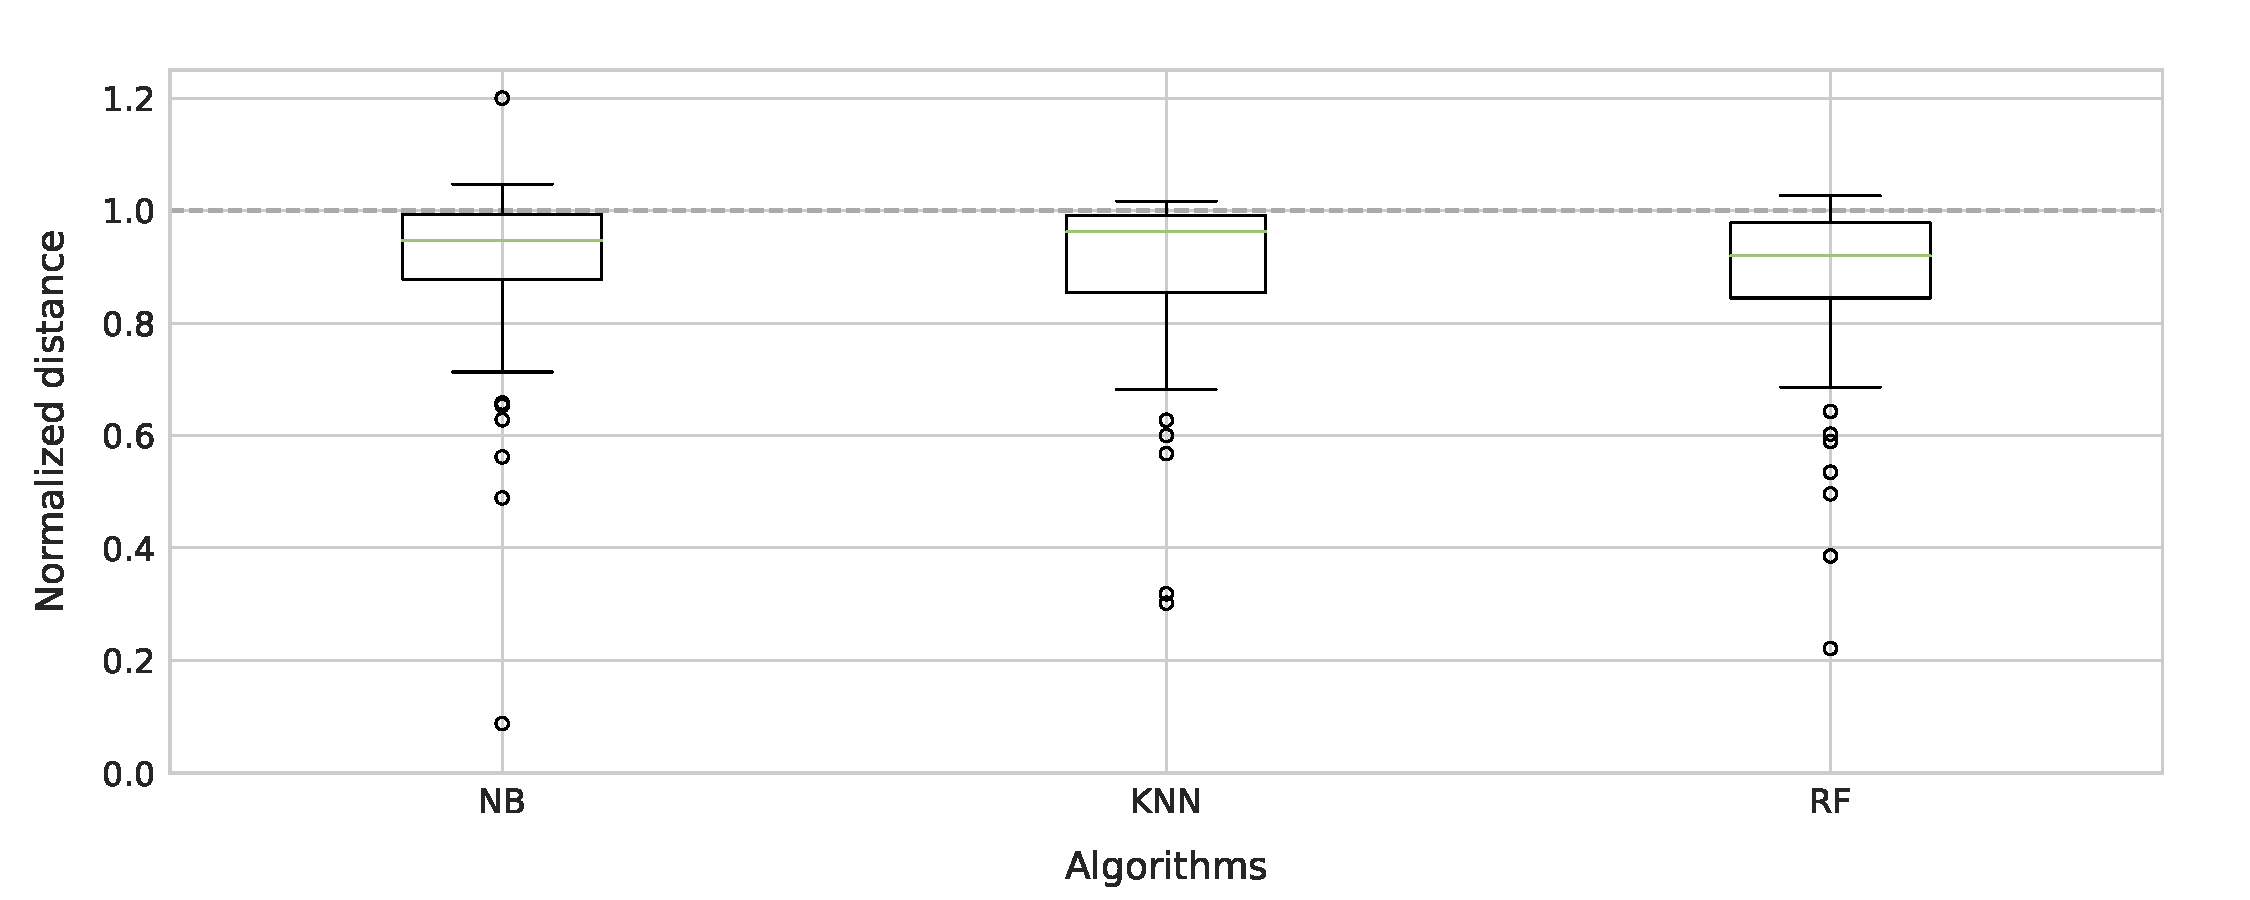
\includegraphics[width=0.7\textwidth]{chapters/data-centric/supervised/img/evaluation2.pdf}
    \caption{Normalized distances between the scores obtained by optimizing our effective prototypes and the ones obtained optimizing the exhaustive set.}
    \label{effective-fig:eval-exhaustive-vs-effective}
\end{figure}

\subsection{Complementing Hyperparameter Optimization with Pre-processing}
\label{effective-sec:eval-dpso-vs-cash}

\begin{figure*}[!t]
	\centering
	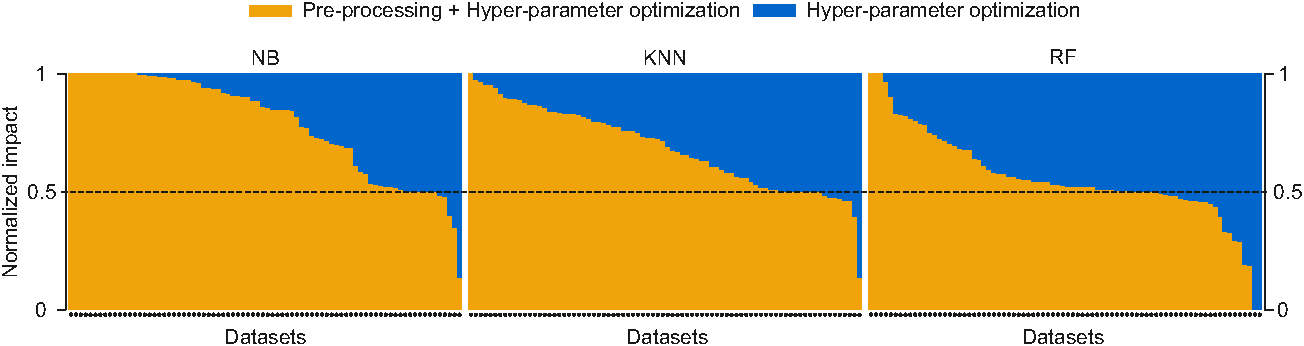
\includegraphics[width=1.0\textwidth]{chapters/data-centric/supervised/img/barplot-10.pdf}
	\caption{The impact of dedicating a portion of the optimization budget to pre-processing compared to using the whole optimization budget for the hyperparameter optimization. \todo{Invertire i colori}}
	\label{effective-fig:eval-pre-processing-hyperparameter}
\end{figure*}

We have just shown that our effective prototypes have similar impact as the exhaustive ones.
Now we want to compare the impact of the effective prototypes against optimizing only the hyperparameters of the ML algorithm.
That is, we want to examine whether dedicating a part of the optimization budget to the pre-processing impacts more (positively) the results of the analysis, than using the whole budget for the hyperparameter optimization\footnote{To enable the application of the ML algorithms on all the datasets, whenever required, we apply the necessary transformation (e.g, imputation or encoding).}.

To this end, for the latter we now dedicate the total optimization budget (i.e., 400 seconds), and for the former, inspired by \cite{Quemy20InfSystems}, we split the budget 50-50 between the pre-processing pipeline optimization and the hyperparameter optimization (i.e., 200 seconds for the pre-processing, and 200 seconds for the hyperparameter optimization).
The time for the pre-processing is further split among the five different pipeline prototypes (i.e., 40 seconds each).

To compare the results, we calculate the impact using the formulas below, which correspond to the normalized distance from either pre-processing or hyperparameter optimization to the maximum improvement that can be achieved, regardless of whether pre-processing is applied or not.

\begin{equation*}
    \text{\textit{pp impact}} = \frac{ACC_{\textup{eff}} - ACC_{\varnothing}}{max(ACC_{\textup{eff}}, ACC_{\textup{hpo}}) - ACC_{\varnothing}}
\end{equation*}

\begin{equation*}
    \text{\textit{hp impact}} = \frac{ACC_{\textup{hpo}} - ACC_{\varnothing}}{max(ACC_{\textup{eff}}, ACC_{\textup{hpo}}) - ACC_{\varnothing}}
\end{equation*}

$ACC_{\varnothing}$ is yet again the baseline performance (i.e., accuracy of the algorithm $A$ with default hyperparameters over the original dataset $\altmathcal{D}$).
$ACC_{\textup{eff}}$ is still the accuracy of our approach, i.e., the optimized algorithm $A_{{\lambda}^{\star}}$ with half of the whole budget over the dataset transformed using the optimized instantiation of the effective set of prototypes (with half of the whole budget).
Finally, $ACC_{\textup{hpo}}$ is the accuracy of the optimized algorithm $A_{{\lambda}^{\star}}$ (i.e, using the entire budget) over the original dataset, formally $ACC_{\textup{hpo}} = ACC(A_{{\lambda}^{\star}}(\altmathcal{D}_{train}), (\altmathcal{D}_{valid}))$.

To obtain relative values that sum to 1, we normalize the impacts dividing them by their sum.
For instance, for the pre-processing score we calculate the following:
\begin{equation*}
    \text{\textit{normalized pp impact}} = \frac{\text{\textit{pp impact}}}
    {\text{\textit{pp impact}} + \text{\textit{hp impact}}}
\end{equation*}


We perform the same for the hyperparameter impact and plot the results obtained for all the algorithms and datasets in \Cref{effective-fig:eval-pre-processing-hyperparameter}, where each bar represents the results obtained for a single dataset.
The different colors represent the impact values of pre-processing and hyperparameter optimization.

Observing the bar charts one can see that (i) dedicating a portion of the budget to pre-processing, brings benefit to the analysis in most of the cases (i.e., $73\%$ of the cases), and (ii) the impact of hyperparameter optimization, increases with the increase of the number of hyperparameters of the ML algorithm (e.g., hyperparameter optimization impacts more RF than NB).
Overall, we can conclude that pre-processing is a critical step that once effectively applied may have a high positive impact on the final result of the analysis.

\section{Conclusions and Future Works}
\label{effective-sec:conclusions}

In this chapter, we first studied the overall impact of pre-processing steps when chained together inside prototypes and then delved into examining the impact of instantiating steps via various transformations.
As a result, we defined a method that allows to generate effective pre-processing pipelines.
That is, pipelines that consist of, (i) compatible pairs of steps concerning the framework used,  (ii) meaningful pairs of steps in terms of general knowledge (best practices), and (iii) promising pairs of steps that once applied are expected to provide higher overall impact (domain knowledge).
In addition, via the meta-learning phase proposed, we aim to guide the pipeline instantiation in order to facilitate finding better transformations.

An extensive evaluation on 80 datasets with heterogeneous characteristics, from sample size to feature types, and a set of classification algorithms (i.e., Naive Bayes, Random Forest, K-Nearest Neighbours), showed that our devised prototypes give promising results.
More specifically, we were able to observe that:
\begin{itemize}
    \item [--] The overall impact of optimizing pre-processing is not negligible and it may boost the performance of the overall analytics (e.g., accuracy).
    \item [--] There is no universal pre-processing prototype that works best for every dataset and algorithm.
    \item [--] With 24 times less time budget, our proposed prototypes were able to obtain results that were as good as 90\% in the median of the optimal ones found through an exhaustive search.
    \item [--] Dedicating a portion of the time to the pre-processing optimization, instead of dedicating it entirely to hyperparameter optimization may boost the final result of the analysis.
	On average, in 73\% of the cases including pre-processing in the optimization, outperformed the results of only optimizing hyperparameters.
\end{itemize}

The results indicate that pre-processing can boost the performance of the ML algorithm.
Hence, it must be considered as an integral part of the data analytics optimization process.

Finally, previous works have shown the effectiveness of meta-learning for solving the cold start problem \cite{Feurer15AAAI}, hence as immediate future work, we intend to extend an optimization framework (i.e., HyperOpt) with a complementary meta-learning module that can ease the cold-start problem, facilitating the search for optimal instantiations.